\PassOptionsToPackage{unicode}{hyperref}
\PassOptionsToPackage{hyphens}{url}

\documentclass[11pt, a4paper]{report}
\usepackage[utf8]{inputenc}
%\usepackage{natbib}
\usepackage{graphicx}
\usepackage[left=2.5cm,top=2.5cm,right=2.5cm,bottom=4cm]{geometry}
%\usepackage[none]{hyphenat}
%\usepackage{showframe}
\usepackage{ragged2e}
\usepackage[english]{babel}
\usepackage{indentfirst}
\usepackage{sectsty}
\usepackage{authblk}
\usepackage{hyperref}
\usepackage{pdfpages}
\usepackage{floatrow}
\usepackage{amsmath,amsfonts,amssymb,amsthm,epsfig,epstopdf,titling,url,array}
\usepackage{mathtools}
\usepackage{tikz, tkz-base, tkz-fct}
\usepackage{mathdesign}
\usepackage{cancel}
\usepackage{dirtytalk}
\usepackage{pgfplots}
\usepackage{tikz}

% KnitR

\usepackage{lmodern}
\usepackage{ifxetex,ifluatex}
\ifnum 0\ifxetex 1\fi\ifluatex 1\fi=0 % if pdftex
\usepackage[T1]{fontenc}
  \usepackage[utf8]{inputenc}
\usepackage{textcomp} % provide euro and other symbols
\else % if luatex or xetex
\usepackage{unicode-math}
\defaultfontfeatures{Scale=MatchLowercase}
\defaultfontfeatures[\rmfamily]{Ligatures=TeX,Scale=1}
\fi
% Use upquote if available, for straight quotes in verbatim environments
\IfFileExists{upquote.sty}{\usepackage{upquote}}{}
\IfFileExists{microtype.sty}{% use microtype if available
	\usepackage[]{microtype}
	\UseMicrotypeSet[protrusion]{basicmath} % disable protrusion for tt fonts
}{}
\makeatletter
\@ifundefined{KOMAClassName}{% if non-KOMA class
	\IfFileExists{parskip.sty}{%
		\usepackage{parskip}
	}{% else
		\setlength{\parindent}{0pt}
		\setlength{\parskip}{6pt plus 2pt minus 1pt}}
}{% if KOMA class
	\KOMAoptions{parskip=half}}
\makeatother
\usepackage{xcolor}
\IfFileExists{xurl.sty}{\usepackage{xurl}}{} % add URL line breaks if available
\IfFileExists{bookmark.sty}{\usepackage{bookmark}}{\usepackage{hyperref}}
\urlstyle{same} % disable monospaced font for URLs
%\usepackage[margin=1in]{geometry}
\usepackage{color}
\usepackage{fancyvrb}
\newcommand{\VerbBar}{|}
\newcommand{\VERB}{\Verb[commandchars=\\\{\}]}
\DefineVerbatimEnvironment{Highlighting}{Verbatim}{commandchars=\\\{\},fontsize=\scriptsize}
% Add ',fontsize=\small' for more characters per line
\usepackage{framed}
\definecolor{shadecolor}{RGB}{248,248,248}
\newenvironment{Shaded}{\begin{snugshade}}{\end{snugshade}}
\newcommand{\AlertTok}[1]{\textcolor[rgb]{0.94,0.16,0.16}{#1}}
\newcommand{\AnnotationTok}[1]{\textcolor[rgb]{0.56,0.35,0.01}{\textbf{\textit{#1}}}}
\newcommand{\AttributeTok}[1]{\textcolor[rgb]{0.77,0.63,0.00}{#1}}
\newcommand{\BaseNTok}[1]{\textcolor[rgb]{0.00,0.00,0.81}{#1}}
\newcommand{\BuiltInTok}[1]{#1}
\newcommand{\CharTok}[1]{\textcolor[rgb]{0.31,0.60,0.02}{#1}}
\newcommand{\CommentTok}[1]{\textcolor[rgb]{0.56,0.35,0.01}{\textit{#1}}}
\newcommand{\CommentVarTok}[1]{\textcolor[rgb]{0.56,0.35,0.01}{\textbf{\textit{#1}}}}
\newcommand{\ConstantTok}[1]{\textcolor[rgb]{0.00,0.00,0.00}{#1}}
\newcommand{\ControlFlowTok}[1]{\textcolor[rgb]{0.13,0.29,0.53}{\textbf{#1}}}
\newcommand{\DataTypeTok}[1]{\textcolor[rgb]{0.13,0.29,0.53}{#1}}
\newcommand{\DecValTok}[1]{\textcolor[rgb]{0.00,0.00,0.81}{#1}}
\newcommand{\DocumentationTok}[1]{\textcolor[rgb]{0.56,0.35,0.01}{\textbf{\textit{#1}}}}
\newcommand{\ErrorTok}[1]{\textcolor[rgb]{0.64,0.00,0.00}{\textbf{#1}}}
\newcommand{\ExtensionTok}[1]{#1}
\newcommand{\FloatTok}[1]{\textcolor[rgb]{0.00,0.00,0.81}{#1}}
\newcommand{\FunctionTok}[1]{\textcolor[rgb]{0.00,0.00,0.00}{#1}}
\newcommand{\ImportTok}[1]{#1}
\newcommand{\InformationTok}[1]{\textcolor[rgb]{0.56,0.35,0.01}{\textbf{\textit{#1}}}}
\newcommand{\KeywordTok}[1]{\textcolor[rgb]{0.13,0.29,0.53}{\textbf{#1}}}
\newcommand{\NormalTok}[1]{#1}
\newcommand{\OperatorTok}[1]{\textcolor[rgb]{0.81,0.36,0.00}{\textbf{#1}}}
\newcommand{\OtherTok}[1]{\textcolor[rgb]{0.56,0.35,0.01}{#1}}
\newcommand{\PreprocessorTok}[1]{\textcolor[rgb]{0.56,0.35,0.01}{\textit{#1}}}
\newcommand{\RegionMarkerTok}[1]{#1}
\newcommand{\SpecialCharTok}[1]{\textcolor[rgb]{0.00,0.00,0.00}{#1}}
\newcommand{\SpecialStringTok}[1]{\textcolor[rgb]{0.31,0.60,0.02}{#1}}
\newcommand{\StringTok}[1]{\textcolor[rgb]{0.31,0.60,0.02}{#1}}
\newcommand{\VariableTok}[1]{\textcolor[rgb]{0.00,0.00,0.00}{#1}}
\newcommand{\VerbatimStringTok}[1]{\textcolor[rgb]{0.31,0.60,0.02}{#1}}
\newcommand{\WarningTok}[1]{\textcolor[rgb]{0.56,0.35,0.01}{\textbf{\textit{#1}}}}
\usepackage{graphicx,grffile}
\makeatletter
\def\maxwidth{\ifdim\Gin@nat@width>\linewidth\linewidth\else\Gin@nat@width\fi}
\def\maxheight{\ifdim\Gin@nat@height>\textheight\textheight\else\Gin@nat@height\fi}
\makeatother
% Scale images if necessary, so that they will not overflow the page
% margins by default, and it is still possible to overwrite the defaults
% using explicit options in \includegraphics[width, height, ...]{}
\setkeys{Gin}{width=0.6\maxwidth,height=0.6\maxheight,keepaspectratio}
% Set default figure placement to htbp
\makeatletter
\def\fps@figure{h!}
\makeatother
\setlength{\emergencystretch}{3em} % prevent overfull lines
\providecommand{\tightlist}{%
	\setlength{\itemsep}{0pt}\setlength{\parskip}{0pt}}
\renewcommand{\baselinestretch}{1.0}

\definecolor{coolblack}{rgb}{0.0, 0.18, 0.39}
%\hypersetup{colorlinks, breaklinks,
%	linkcolor=coolblack,
%	filecolor=[rgb]{0.19, 0.55, 0.91},      
%	urlcolor=[rgb]{0.19, 0.55, 0.91},
%	anchorcolor=[rgb]{0.19, 0.55, 0.91},
%	citecolor=black%}

\newcommand{\indep}{\perp \!\!\! \perp}
\newcommand{\nindep}{\not\!\perp\!\!\!\perp}

\let\origfigure\figure
\let\endorigfigure\endfigure



\theoremstyle{plain}
\newtheorem{thm}{Theorem}[section]
\newtheorem{lem}[thm]{Lemma}
\newtheorem{prop}[thm]{Proposition}
\newtheorem*{cor}{Corollary}

\theoremstyle{plain}
\newtheorem{defn}{Definition}[section]
\newtheorem{conj}{Conjecture}[section]
\newtheorem{exmp}{Example}[section]

\theoremstyle{remark}
\newtheorem*{rem}{Remark}
\newtheorem*{note}{Note}





\title{\Huge \textbf{Econometrics II} \\ \LARGE Notes - Midterm}
\author{\Large William Radaic Peron}
\affil{\Large EESP-FGV}

%\sectionfont{\fontsize{12}{12}\selectfont}
%\chapterfont{\fontsize{16}{12}\selectfont}
%\subsectionfont{\fontsize{11}{11}\selectfont}

\begin{document}
\setlength{\parindent}{0em}
%\setlength{\parskip}{0.6em}
\maketitle

\tableofcontents

\chapter{Introduction}

\section{Motivation}

This course will be dedicated to \textit{time series analysis.} Informally, a \textit{time series} is any type of data collected over time -- or, more formally, it is the realization of a stochastic process indexed in time. We usually denote the time series as follows: 
$$ y_1, ..., y_T; \hspace{1em} \{y_t\}_{i=1}^T; \hspace{1em} \{y_t\}_t $$

Time series analysis is useful for a number of different applications: 
\begin{itemize}
	\item \textbf{Forecasting.} \begin{itemize}
		\item Uni and multivariate models 
		\item \textbf{ARIMA} models: mean and confidence interval forecasting
		\item \textbf{ARCH} models: variance forecasting -- especially useful in finance for volatility and risk
	\end{itemize}
	\item \textbf{Dynamics.} Evaluate the impact of one variable in another over time. \begin{itemize}
		\item Multivariate models including VAR, ECM
		\item Contemporaneous lagged structural relations
	\end{itemize}
\end{itemize}

It is important to address a first and simple question. \textbf{Why time series are different from other data?} The answer is also simple but incredibly relevant: \textit{time series observations are not serially independent!}
$$ Y_t \nindep Y_{t-j} $$
In fact, they don't even have to be identically distributed:
$$ F_{Y_t} \neq F_{Y_{t-j}} $$
This means that the essential \textit{iid} hypothesis for traditional Econometrics \textit{does not hold.} This means that we'll have to make some adjustments to our methods. That is the task of time series analysis.

\section{Statistics with dependence}

Let's begin with a proper definition of a time series. 

\subsection{Definition of a time series}

Suppose that we have a probability space $(\Omega, S, \mathbb{P})$. $\Omega$ is the sample space; $S$ is the set of all events; $\mathbb{P}$ is a measure of probability $\mathbb{P}: S \rightarrow [0,1]$. From this, we define a random variable $Y: \Omega \rightarrow \mathbb{R}$. A realization of this r.v. is denoted by $y = Y(\omega)$ with fixed $\omega$.

From this, we can define multiple random variables in the same sample space, indexed by integers:
$$	Y = \{..., Y_{t-2}, Y_{t-1}, Y_t, ...\} $$
This is equivalent to writing:
$$ Y: \Omega x \mathbb{Z} \rightarrow \mathbb{R}$$

We now arrive at our formal definition of a time series: $\{Y_t, t \in \mathbb{Z} \}$ is a time-indexed stochastic process.
\begin{itemize}
	\item $Y(\cdot, t): \Omega \rightarrow \mathbb{R}$ is a r.v. for fixed $t$.
	\item $Y(\omega, \cdot): \mathbb{Z} \rightarrow \mathbb{R}$ is a \textit{sequence of real numbers} for a fixed $\omega$. In other words, this represents the \textit{observed time series.}
	\item For fixed $t, \omega$, $Y(\omega, t) \in \mathbb{R}$.
\end{itemize}

\subsection{Unconditional expectation}

An important concept to make clear here is \textit{unconditional expectation.} With fixed $t$, 
$$ \mathbb{E}(Y_t) = \int_{-\infty}^{\infty} x f_{Y_t}(x) dx $$
Note the $Y_t$ subscript on the probability density function $f_{Y_t}$. This means that $\mathbb{E}(Y_t)$ is not calculated with the values assumed by $Y_{t-1}, Y_{t+1}$. This raises an important problem: \textit{how would you be able to estimate $\mathbb{E}(Y_t)$?} Note that we only observe $Y_t = y_t$, i.e., one realization of the r.v.


\subsection{Statistical dependence}

For any random variables $X, Y$, we can define multiple measures of dependency:
\begin{itemize}
	\item \textbf{Linear:} $Cov(X,Y) \equiv \mathbb{E}(XY) - \mathbb{E}(X)\mathbb{E}(Y) $
	\item \textbf{Quadratic:} $Cov(X^2, Y^2)$
	\item \textbf{General:} $Cov(f(X), g(Y))$. This is a measure of covariance between two general functional forms of $X$ and $Y$.
\end{itemize}
With this general definition, we arrive at an equivalent definition for independent random variables:
\begin{itemize}
	\item $F_{X,Y}(x,y) = F_X(x) * F_Y(y),$ i.e., joint pdf is equal to the product of the marginal pdfs.
	\item $Cov(f(X), g(Y)) = 0$ for every pair of bounded functions $f, g$.
\end{itemize}

From this, we now define the \textit{autocovariance and autocorrelation functions.}

\begin{defn}
	$\gamma_{j,t} := Cov(Y_t, Y_{t-j})$ is the \textbf{autocovariance function} for a given time series $\{Y_t, t \in \mathbb{Z} \}.$
\end{defn}

\begin{defn}
	$\rho_{j,t} := \dfrac{\gamma_{j,t}}{\sqrt{\gamma_{0,t}\gamma_{0,t-j}}}$ is the \textbf{autocorrelation function} for a given time series $\{Y_t, t \in \mathbb{Z} \}.$
\end{defn}

Note that, if \textit{iid} holds:
$$ \gamma_{j,t} = \begin{cases}
	0 & j \neq 0, \forall t \\
	Var(Y) & otherwise 
\end{cases} $$

This is an example of an autocorrelation function.

\begin{figure}[h!]
	\centering
	\includegraphics[width=0.6\linewidth]{"acf example"}
	%\caption{}
	\label{fig:acf-example}
\end{figure}

\section{Asymptotic theory with dependence}

Some form of asymptotic theory is needed to enable \textit{any kind of statistical analysis.} Namely, we need to have some form of Law of Large Numbers (LLN) and Central Limit Theorem (CLT) that are analogous to the \textit{iid} environment. This will be achieved in our setting with some conditions called \textit{stationarity} and \textit{ergodicity.}

\subsection{Stationarity}

\begin{defn}
	A process $\{Y_t, t \in \mathbb{Z} \}$ is \textbf{strictly stationary} if, for all finite set of indexes $\{t_1, ..., t_r\}$ and for all $m \in \mathbb{Z}$, $F(y_{t_1},..., y_{t_r}) = F(y_{t_1+m},..., y_{t_r+m})$ holds, where $F(y_{t_1},..., y_{t_r})$ is the joint cdf of $(Y_{t_1},..., Y_{t_r}).$
\end{defn}

More informally, a given process is called \textit{strictly stationary} if its statistical properties depend only on the \textit{relative position} between observations, and not its \textit{absolute position.}

We'll usually adopt a weaker definition of stationarity for our models. Henceforth, we will refer to stationarity in this sense.

\begin{defn}
	A process $\{Y_t, t \in \mathbb{Z} \}$ is \textbf{stationary} (or weakly stationary) if there exists $\mu \in \mathbb{R}$ and $\{\gamma_j\}_{j \in \mathbb{N}}$ such that:
	\begin{itemize}
		\item $\mathbb{E}(Y_t) = \mu, \hspace{1em} \forall t$
		\item $\mathbb{E}[(Y_t - \mu)(Y_{t-j}-\mu)] = \gamma_j, \hspace{1em} \forall (t,j) \in \mathbb{N}^2$
	\end{itemize}
\end{defn}

	Note that, from the second condition in the definition, we have $\mathbb{E}(Y_t - \mu)^2 = \gamma_0 \in \mathbb{R}, \forall t \in \mathbb{N}.$ In other words, \textit{the unconditional variance of the time series is constant.}

\vspace{1em}

Some important remarks on stationarity: 
\begin{itemize}
	\item Stationarity does not imply strict stationarity
	\item Stricy stationarity does not imply stationarity
	\item Every strictly stationary process with finite variance is stationary
	\item Every iid process is strictly stationary
	\item Every strictly stationary process is identically distributed
	\item A stationary process is not necessarily identically distributed
\end{itemize}

\subsection{Ergodicity}

Stationarity is not enough to guarantee that we have even a Law of Large Numbers. To see why that is the case, consider the following example:
$$ Y_t = X + \varepsilon_t, \hspace{1em} \varepsilon \sim \mathcal{N}(0, \sigma^2), \hspace{1em} X \sim \mathcal{N}(0,1), \hspace{1em} X \indep \varepsilon_t $$

Is this process stationary? No, because the sample \textit{time average} $\bar{y} = \frac{1}{T}\sum_{t=1}^T y_t$ does not converge to the population \textit{ensemble average} $\mathbb{E}(Y_t) = \mu$.

We need some condition that guarantees that the dependence structure of the time series decays as the observation get further from each other. That is the intuition behind \textit{ergodicity.}

\begin{defn}
	A strictly stationary process $\{Y_t, t \in \mathbb{Z} \}$ is called \textbf{ergodic} if
	$$ \lim_{J \rightarrow \infty} \dfrac{1}{J} \sum_{j=1}^J Cov[f(X_1), g(X,j)] = 0, $$
	for all pairs of bounded functions $f, g$.
\end{defn}

This is a kind of mean asymptotic independence, in which the asymptotic independence would be defined by $Cov[f(X_1), g(X_J)] \rightarrow 0$ as $J \rightarrow \infty$. 

Now, we can define a Law of Large Numbers -- also called the \textit{Ergodic Theorem}.

\begin{thm}
	Given an ergodic stochastic process $\{Y_t, t \in \mathbb{Z} \}$ such that $\mathbb{E}|Y_1| < \infty$,
	$$\lim_{T \rightarrow \infty} \dfrac{1}{T} \sum_{t=1}^T Y_t = \mathbb{E}(Y_1) \hspace{1em} almost \, sure$$
\end{thm}

This theorem is the generalization of the strong LLN. However, it presupposes \textit{strict stationarity,} which is a very strong assumption most of the time. Fortunately, this theorem gave rise to other definitions that arrive at our objective, namely, a LLN for the first two moments.

\begin{defn}
	A stationary process $\{Y_t, t \in \mathbb{Z} \}$ is said to be \textbf{ergodic for the mean} if
	$$ \dfrac{1}{T} \sum_{t=1}^T Y_t \to_p \mathbb{E}(Y_t), \hspace{1em} T \to \infty $$
\end{defn}

\begin{defn}
	A stationary process $\{Y_t, t \in \mathbb{Z} \}$ is said to be \textbf{ergodic for the second moment} if, for every $j,$
	$$ \dfrac{1}{T-j} \sum_{t=j+1}^T Y_t Y_{t-j} \to_p \mathbb{E}(Y_t), \hspace{1em} T \to \infty $$
\end{defn}

\begin{prop}
	$\sum_{j=0}^{\infty} |\gamma_j| < \infty $ is a suficient condition for ergodicity for the mean.
\end{prop}

\begin{proof}
	Let $Z_t := Y_t - \mu$ and $\bar{Z_t} := \frac{1}{T} \sum_{t=1}^T Z_t$, where $\{Y_t, t \in \mathbb{Z} \}$ is a stationary process. We will show that $\bar{Z_t}$ converges to 0 in mean square.
	
	\begin{math}
		\begin{aligned}
			\mathbb{E}\left(\bar{Z}_{T}^{2}\right) &=\mathbb{E}\left[\left(\frac{1}{T} \sum_{t=1}^{T} Z_{t}\right)\left(\frac{1}{T} \sum_{t=1}^{T} Z_{t}\right)\right]=\frac{1}{T^{2}} \mathbb{E}\left(\sum_{s=1}^{T} \sum_{t=1}^{T} Z_{s} Z_{t}\right) \\
			&=\frac{1}{T^{2}} \sum_{s=1}^{T} \sum_{t=1}^{T} \mathbb{E}\left(Z_{s} Z_{t}\right)=\frac{1}{T^{2}} \sum_{s=1}^{T} \sum_{t=1}^{T} \gamma_{s-t}=\frac{1}{T} \sum_{j=-T+1}^{T-1} \frac{T-|j|}{T} \gamma_{j} \\
			& \leq \frac{1}{T} \sum_{j=-T+1}^{T-1} \frac{T-|j|}{T}\left|\gamma_{j}\right| \leq \frac{1}{T} \sum_{j=-T+1}^{T-1}\left|\gamma_{j}\right| \rightarrow 0
		\end{aligned}
	\end{math} 

\end{proof}

\subsection{A Central Limit Theorem for time series}

The conditions that guarantee the existence of a CLT for stationary and ergodic processes are much more envolving than in the \textit{iid} environment. However, we have a relatively simple result that will be useful to us in time series analysis. It will now be presented without proof.

\begin{thm}
	Let $\{Y_t, t \in \mathbb{Z} \}$ be a \textbf{linear} stationary process, i.e., that can be written in the form $Y_t = \mu + \sum_{j=0}^{\infty} \psi_j \epsilon_{t-j}$, where $\varepsilon \sim_{iid} (0, \sigma^2)$ and $\sum_{j = -\infty}^{\infty} | \psi_j | < \infty$. Then,
	$$ \sqrt{T}(\bar{Y_t}-\mu) \to_d \mathcal{N}(0, \omega^2), $$ 
	where $\omega^2 := \sum_{j = -\infty}^{\infty} \gamma_{j} < \infty $	
\end{thm}

\chapter{ARMA Models}

ARMA is a class of models that we'll employ frequently in time series analysis. Let's begin with some definitions.

\section{White noise}

We call \textit{white noise} stationary time series with mean zero that do not have serial correlation. 

\begin{defn}
	$\{Y_t, t \in \mathbb{Z} \}$ is \textbf{white noise}, denoted by $Y_t \sim wn(0,\sigma^2)$, if
	$$\mathbb{E}\left(Y_{t}\right)=0 ; \quad \mathbb{E}\left(Y_{t}, Y_{t-j}\right)=\left\{\begin{array}{ll}
		\sigma^{2} & j=0 \\
		0 & j \neq 0
	\end{array}\right.$$
\end{defn}

This is the most simple time series -- except for the \textit{iid} case, where independence also holds. It will be the building block for a number of processes that we will study.

\section{Moving Average processes}

Let's begin with the simplest form of MA processes: MA(1). 
\begin{defn}
	A stationary process $\{Y_t, t \in \mathbb{Z} \}$ is called \textbf{MA(1)}, or a \textbf{moving average of order 1}, if it follows the following form:
	$$ Y_t = c + \varepsilon_t + \theta \varepsilon_{t-1}, \hspace{1em} \varepsilon_t \sim wn(0, \sigma^2), $$
	where $c, \theta$ are constant.
\end{defn}

\subsection{Moments of an MA(1) model}

The expected value of an MA(1) is:
$$
\mu \equiv \mathbb{E}\left(Y_{t}\right)=\mathbb{E}\left(c+\varepsilon_{t}+\theta \varepsilon_{t-1}\right)=c
$$

With this result, we can rewrite the model as: 
$$
\left(Y_{t}-\mu\right)=\varepsilon_{t}+\theta \varepsilon_{t-1}
$$

Multiplying both sides by $\left(Y_{t-j}-\mu\right)$ yields:
$$
\begin{aligned}
	\left(Y_{t}-\mu\right)\left(Y_{t-j}-\mu\right) &=\left(\epsilon_{t}+\theta \epsilon_{t-1}\right)\left(\epsilon_{t-j}+\theta \epsilon_{t-j-1}\right) \\
	&=\epsilon_{t} \epsilon_{t-j}+\theta \epsilon_{t} \epsilon_{t-j-1}+\theta \epsilon_{t-1} \epsilon_{t-j}+\theta^{2} \epsilon_{t-1} \epsilon_{t-j-1}
\end{aligned}
$$

Applying the expected value operator to both sides, we have the autocovariances of the model.
$$
\gamma_{j} \equiv \mathbb{E}\left[\left(Y_{t}-\mu\right)\left(Y_{t-j}-\mu\right)\right]=\left\{\begin{array}{ll}
	\left(1+\theta^{2}\right) \sigma^{2} & j=0 \\
	\theta \sigma^{2} & j=\pm 1 \\
	0 & |j|>1
\end{array}\right.
$$

\subsection{Some examples of MA(1) processes}

\begin{figure}[h!]
	\centering
	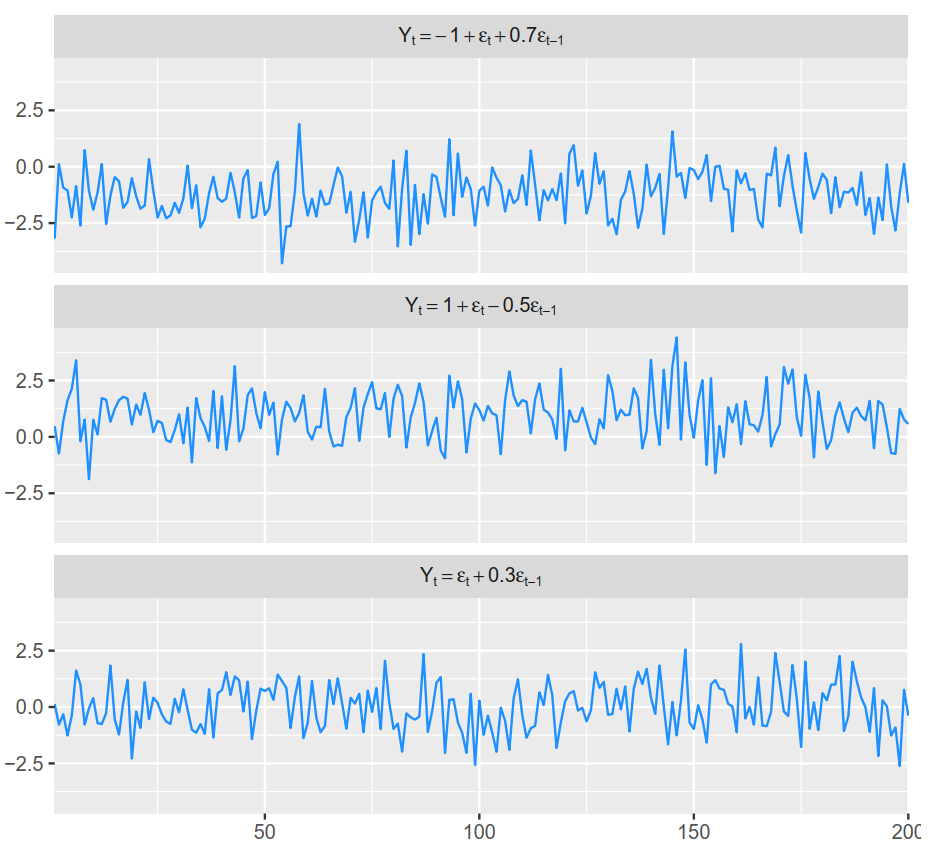
\includegraphics[width=0.6\linewidth]{ma1}
	\label{fig:ma1}
\end{figure}

\subsection{Deriving the Autocorrelation function of the MA(1) process}

While deriving the moments of the MA(1), it became clear that the process is stationary and ergodic to the mean. Note that the time average $\bar{y_t}$ converges to $\mathbb{E}(Y_t)$, the \textit{ensemble average}, the absolute sum of all covariances is clearly finite ($\gamma_j = 0, \forall j > 1$) and the dependence structure depends only on the relative positions of the observations.

Let's use the results of the autocovariances to construct the ACF:

$$\rho_{j} \equiv \frac{\gamma_{j}}{\gamma_{0}}=\left\{\begin{array}{ll}
	1 & j=0 \\
	\frac{\theta}{1+\theta^{2}} & j=\pm 1 \\
	0 & |j|>1
\end{array}\right.$$

Note that the ACF of an MA(1) process is \textit{truncated} in zero for lags greater than 1.

\begin{figure}[h!]
	\centering
	\includegraphics[width=0.6\linewidth]{"fac facp"}
	\label{fig:fac-facp}
\end{figure}

\section{Generalizing the MA model}

We can now generalize the MA(1) model for a moving average of order $q$.

\begin{defn}
	A stationary process $\{Y_t, t \in \mathbb{Z} \}$ is called \textbf{MA(q)}, or a \textbf{moving average of order q}, if it follows the following form:
	$$ Y_t = c + \varepsilon_t + \theta_1 \varepsilon_{t-1} + ... + \theta_q \varepsilon_{t-q}, \hspace{1em} \varepsilon \sim wn(0, \sigma^2), $$
	where $c, \theta_1, ..., \theta_q \in \mathbb{R}, q \in \mathbb{Z}^+$.
\end{defn}

\subsection{Moments of an MA(q) process}

The expected value of an MA(q) is:
$$
\mu \equiv \mathbb{E}\left(Y_{t}\right)=\mathbb{E}\left(c+\varepsilon_{t}+\theta_{1} \varepsilon_{t-1}+\cdots+\theta_{q} \varepsilon_{t-q}\right)=c
$$

Again, using the first result, we can rewrite the model as:
$$
\left(Y_{t}-\mu\right)=\varepsilon_{t}+\theta_{1} \varepsilon_{t-1}+\cdots+\theta_{q} \varepsilon_{t-q}
$$

Multiplicando ambos os lados por $\left(Y_{t-j}-\mu\right),$ temos
$$
\begin{aligned}
	\left(Y_{t}-\mu\right)\left(Y_{t-j}-\mu\right) &=\left(\sum_{k=0}^{q} \theta_{k} \varepsilon_{t-k}\right)\left(\sum_{k=0}^{q} \theta_{k} \varepsilon_{t-j-k}\right) \\
	&=\sum_{k=0}^{q} \sum_{\ell=0}^{q} \theta_{k} \theta_{\ell} \varepsilon_{t-k} \varepsilon_{t-j-\ell},
\end{aligned}
$$

where $\theta_{0}=1 .$ Applying the expectation operator, we have:
$$
\gamma_{j}=\left\{\begin{array}{ll}
	\left(\theta_{j}+\theta_{j+1} \theta_{1}+\theta_{j+2} \theta_{2}+\cdots+\theta_{q} \theta_{q-j}\right) \sigma^{2} & |j|=0,1, \ldots, q \\
	0 & |j|>q
\end{array}\right.
$$

\subsection{Deriving the Autocorrelation function of the MA(q) process}

Again, we can clearly see that the MA(q) model is \textit{stationary} and \textit{ergodic.} Note that the time average $\bar{y_t}$ converges to $\mathbb{E}(Y_t)$, the \textit{ensemble average}, the absolute sum of all covariances is clearly finite ($\gamma_j = 0, \forall j > q$) and the dependence structure depends only on the relative positions of the observations.

The autocorrelation function is given by:
$$\rho_{j} \equiv \frac{\gamma_{j}}{\gamma_{0}}=\left\{\begin{array}{ll}
	1 & j=0 \\
	\frac{\theta_{j}+\theta_{j+1} \theta_{1}+\theta_{j+2} \theta_{2}+\cdots+\theta_{q} \theta_{q-j}}{1+\theta_{1}^{2}+\cdots+\theta_{q}^{2}} & |j|=1,2, \ldots, q \\
	0 & |j|>q
\end{array}\right.$$

Now, the ACF is truncated in zero for lags \textit{greater than $q$.}


\section{The MA($\infty$) model}

Consider a special case of a MA(q) model where $q \to \infty$. This yields a moving average of infinite order, MA($\infty$).

\begin{defn}
	A stationary process $\{Y_t, t \in \mathbb{Z} \}$ is called \textbf{MA($\infty$)}, or a \textbf{moving average of infinite order}, if it follows the following form:
	$$ Y_t = c + \sum_{i=0}^{\infty} \theta_i \varepsilon_{t-i}, \hspace{1em} \sim wn(0, \sigma^2), $$
	where $c, \theta_1, ..., \theta_q \in \mathbb{R}, \theta_0 = 1$.
\end{defn}

We also assume that $\sum_{i=0}^{\infty} | \theta_i | < \infty $. This guarantees that the process is \textit{ergodic.}\footnote{Details in Hamilton (1994), Appendix, 3.A.} With this assumption, we can obtain the moments of the MA($\infty$) simply by taking the limit of the finite case MA(q) -- because it enables us to exchange the order between the sum and the expectation operator.

This means that $\mu = c$, as in the previous cases, and:
$$\gamma_{j}=\left(\sum_{i=0}^{\infty} \theta_{j+i} \theta_{i}\right) \sigma^{2}$$

\section{The Wold Decomposition}

This result motivates all ARMA models. It can be defined informally as ``any stationary process has a MA($\infty$) representation''.

\begin{thm}{\textbf{Wold Representation Theorem.}}
	Any process $\{Y_t, t \in \mathbb{Z} \}$ purely nondeterministic can be written as
	$$ Y_t = \mu + \sum_{j=0}^{\infty} \psi_j \varepsilon_{t-j}, $$
	where $\varepsilon_{t} = Y_t - \pi(Y_t | 1, Y_{t-1}, Y_{t-2}, ...)$, i.e., $\varepsilon_{t}$ is the \textit{error of the linear projection of $Y_t$ in $(1, Y_{t-1}, Y_{t-2}, ...)$}.
\end{thm}

\section{Autoregressive models}

Again, we'll begin with its simplest form, AR(1).

\begin{defn}
	A stationary process $\{Y_t, t \in \mathbb{Z} \}$ is called \textbf{AR(1)}, or an \textbf{autoregressive process of order 1}, if it follows the following form:
	$$ Y_t = c + \phi Y_{t-1} + \varepsilon_t, \hspace{1em} \varepsilon_t \sim wn(0, \sigma^2), $$
	where $c, \theta$ are constant.
\end{defn}

\subsection{Moments of an AR(1) process}

With AR($\cdot$) models, we will work in the opposite direction when it comes to stationarity. We'll first \textit{assume} that is holds, and then provide reasoning for why the assumption is valid.

With the assumption of stationarity, we can take expectations and variances on both sides:
$$ \mu = c + \phi \mu \iff \mu = \mathbb{E}(Y_t) = \dfrac{c}{1 - \phi} $$
$$ \gamma_{0} = \phi^2 \gamma_{0} + \sigma^2 \iff \gamma_{0} = Var(Y_t) = \dfrac{\sigma^2}{1 - \phi^2} $$

Using the first result, we can rewrite the model as:
$$ (Y_t - \mu) = \phi (Y_{t-1} - \mu) + \varepsilon_{t} $$

Multiplying both sides by $(Y_{t-j} - \mu)$ and taking expectations yields:
$$ \gamma_{j} = \phi \gamma_{t-j}, \hspace{1em} = 1,2,... $$

\subsection{Some examples of AR(1) series}

\begin{figure}[h!]
	\centering
	\includegraphics[width=0.6\linewidth]{"ar1"}
	\label{fig:fac-facp}
\end{figure}

\subsection{Autocorrelation function of an AR(1) process}

Given that $\gamma_{j} = \phi \gamma_{t-j}$, it is easy to see that the autocovariance is given by:
$$ \gamma_j = \phi^{|j|} \gamma_0, \hspace{1em} j \in \mathbb{Z} $$

Therefore, $\rho_{j} = \dfrac{\gamma_{j}}{\gamma_{0}} = \phi^{|j|}$.

\subsection{Partial Autocorrelation Function}

Note that $Y_t, Y_{t-2}$ \textit{are correlated.} Can we isolate the correlation between $Y_t, Y_{t-2}$ from the effects of $Y_{t-1}$? 
$$ Cor(Y_t, Y_{t-2} | Y_{t-1}) = Cor(c + \phi Y_{t-1} + \varepsilon_{t}, Y_{t-2} | Y_{t-1}) = 0 $$

This is the intuition behind the \textit{partial autocorrelation function} (PACF). 

\begin{defn}
	The \textbf{partial autocorrelation function} of a stationary process $\{Y_t, t \in \mathbb{Z} \}$ is given by:
$$\alpha_{j}=\left\{\begin{array}{ll}
	\operatorname{Cor}\left(Y_{t}, Y_{t-1}\right)=: \rho_{1} & j=1 \\
	\operatorname{Cor}\left(Y_{t}, Y_{t-j} \mid Y_{t-1}, \ldots, Y_{t-j+1}\right) & j \geq 2
\end{array}\right.$$
\end{defn}

To estimate the ACF of a given time series, we need to use its sample equivalent and a version of the Law of Large Numbers, presented in the previous section, because we're only looking for correlations -- i.e., population moments. To estimate the PACF, that is not enough. We're now looking for \textit{partial correlation.} 

It so happens that OLS gives us the \textit{ceteris paribus} effects. Note that a general form for $\beta$ is given by: $ \beta = \frac{Cov(X,Y)}{Var(X)}$. Therefore, we can estimate using OLS the following models for every $j$: 
$$ Y_t = \beta_0 + \beta_1 Y_{t-1} + ... + \alpha_j Y_{t-j} + u_t $$
The last coefficient of \textit{each regression}, $\hat{\alpha}_j$, is a consistent estimator for $\alpha_{j}$. It is important to highlight, here, that a new model shall be estimated \textit{for each $j$}, as it guarantees that the coefficient $\alpha_{j}$ will be conditional on all $t$ \textit{prior} to $j$.

The following plots showcase ACFs and PACFs for AR(1) processes.

\begin{figure}[h!]
	\centering
	\includegraphics[width=0.6\linewidth]{"fac facp ar1"}
	\label{fig:fac-facp-ar1}
\end{figure}

\subsection{Conditions for stationarity}

When is an AR(1) process stationary? Note that:

$$
\begin{aligned}
	Y_{t} &=c+\phi Y_{t-1}+\varepsilon_{t} \\
	&=c+\phi\left(c+\phi Y_{t-2}+\varepsilon_{t-1}\right)+\varepsilon \\
	&=c+\phi\left(c+\phi\left(c+\phi Y_{t-3}+\varepsilon_{t-2}\right)+\varepsilon_{t-1}\right)+\varepsilon_{t} \\
	& \cdots \\
	&=c \sum_{j=0}^{k-1} \phi^{j}+\phi^{k} Y_{t-k}+\sum_{j=0}^{k-1} \phi^{j} \varepsilon_{t-j}
\end{aligned}
$$

Assuming that $|\phi|<1$ and taking the limit $k \rightarrow \infty,$ we have:

$$
Y_{t}=\frac{c}{1-\phi}+\sum_{j=0}^{\infty} \phi^{j} \varepsilon_{t-j}
$$

The first term follows from the sum of an infinite geometric sequence. This means that \textit{an AR(1) process can be written as a MA($\infty$)} with $\sum_{j = 0}^\infty | \theta_j | < \infty$. Note that this is equivalent to saying that the Wold Representation Theorem holds, with $\mu = \frac{c}{1 - \phi}$, $\psi_j = \phi^j$. This guarantees that the AR(1) process is \textit{stationary} and \textit{ergodic.}

\section{Generalizing the AR model}

\begin{defn}
	A stationary process $\{Y_t, t \in \mathbb{Z} \}$ is called \textbf{AR(p)}, or an \textbf{autoregressive process of order p}, if it follows the following form:
	$$ Y_t = c + \phi Y_{t-1} + ... + \phi_p Y_{t-p} + \varepsilon_t, \hspace{1em} \varepsilon_t \sim wn(0, \sigma^2), $$
	where $c, \theta_1, ..., \theta_p$ are constant.
\end{defn}

\subsection{Moments of an AR(p) process}

Assuming stationarity, we can apply again expectations on both sides:
$$
\mu=c+\phi_{1} \mu+\cdots+\phi_{p} \mu \Longleftrightarrow \mu=\frac{c}{1-\phi_{1}-\cdots-\phi_{p}}
$$

Using this result, we can rewrite the model as:
$$
\left(Y_{t}-\mu\right)=\phi_{1}\left(Y_{t-1}-\mu\right)+\cdots+\phi_{p}\left(Y_{t-p}-\mu\right)+\epsilon_{t}
$$

Multiplying both sides by $\left(Y_{t-j}-\mu\right)$ and taking expectations, we have:
$$
\gamma_{j}=\left\{\begin{array}{ll}
	\phi_{1} \gamma_{j-1}+\cdots+\phi_{p} \gamma_{j-p} & j=1,2, \ldots \\
	\phi_{1} \gamma_{1}+\cdots+\phi_{p} \gamma_{p}+\sigma^{2} & j=0
\end{array}\right.
$$
Note that the last term in $\gamma_{0}$ is implied by $\mathbb{E}\left(\epsilon_{t}\right)\left(Y_{t}-\mu\right)=\sigma^{2}$.

\subsection{ACF of an AR(p) process}

Dividing the previous result by $\gamma_{0}$ yields:
$$ \rho_j = \phi_1 \rho_{j-1} + ... + \phi_p \rho_{j-p} $$

Evaluating at $j = 1,2,..., p - 1$ and using $p_i = p_{-i}$, we have the following system of difference equations (aka. Yule-Walker Equations):
$$\left\{\begin{array}{l}
	\rho_{1}=\phi_{1}+\phi_{2} \rho_{1}+\cdots+\phi_{p} \rho_{p-1} \\
	\rho_{2}=\phi_{1} \rho_{1}+\phi_{2}+\cdots+\phi_{p} \rho_{p-2} \\
	\vdots \\
	\rho_{p}=\phi_{1} \rho_{p-1}+\phi_{2} \rho_{p-2}+\cdots+\phi_{p}
\end{array}\right.$$

To solve this, we need to find $\rho_1, \rho_2, ..., \rho_j$ as functions of $\phi_1, \phi_{2}, ..., \phi_j$. The first equation above implies that further correlations from lag $j$ will decay exponentially\footnote{Review this.}. This means that the ACF pattern of an AR(p) looks like the one from the simple AR(1) model.

\section{The Lag Operator}

\begin{defn}
	Given a process $\{Y_t, t \in \mathbb{Z} \},$ the \textbf{lag operator} is defined by:
$$\begin{array}{l}
	L Y_{t}:=Y_{t-1} \\
	L^{2} Y(t):=L\left(L Y_{t}\right)=L\left(Y_{t-1}\right)=Y_{t-2} \\
	\vdots \\
	L^{j} Y(t):=L\left(L\left(L \ldots L Y_{t}\right)=Y_{t-j}\right.
\end{array}$$
\end{defn}

The lag operator is also commutative with multiplication and distributive with regards to addition:
$$ L(cY_t) = c(LY_t) $$
$$ L(Y_t + X_t) = LY_t + LX_t $$

\subsection{The lag operator as a polynomial}

Note that we can use the lag operator as a \textit{polynomial.} We can now rewrite an AR(p) with zero mean as:
$$ (1 - \phi_1 L - \phi_2 L^2 - ... - \phi_p L^p)Y_t = \varepsilon_{t} $$

Note that the term multiplying $Y_t$ \textit{is a polynomial in L.} We denote this by:
$$ (L) Y_t = \varepsilon_{t} $$

Analogously, we can rewrite an MA(q) process as:
$$\begin{aligned}
	Y_{t} &=\epsilon_{t}+\theta_{1} \epsilon_{t-1}+\theta_{2} \epsilon_{t-2}+\cdots+\theta_{q} \epsilon_{t-q} \\
	&=\left(1+\theta_{1} L+\theta_{2} L^{2}+\cdots+\theta_{q} L^{q}\right) \epsilon_{t} \\
	& \equiv \Theta_{q}(L) \epsilon_{t}
\end{aligned}$$

We would also like to define an operator $(1 - \phi L)^{-1}$ such that:
$$ (1 - \phi L)^{-1} (1 - \phi L) = 1 $$

$(1 - \phi L)^{-1}$ is well defined when $|\phi| < 1$ and the following condition holds\footnote{Hamilton (1994), p. 27-29.}:
$$ (1 - \phi L)^{-1} := 1 + \phi L + \phi^2 L^2 + \phi^3 L^3 + ... $$

From this, we can rewrite the AR(1) as a MA($\infty$) by multiplying the AR by $(1 - \phi L)^{-1}$ on both sides:
$$ Y_t = (1 - \phi L)^{-1} \varepsilon_{t}$$

The $(1 - \phi L)^{-1}$ operator will be very useful to translate models between AR and MA representations, aside from highlighting the conditions of stationarity for the process.


\subsection{Stationarity and the lag operator}

We can factor out the polynomial of an AR(p) process as:
$$ 1 - \phi_1 L - ... - \phi_{p} L^p = (1 - \lambda_1 L)...(1 - \lambda_p L), $$
where $\lambda_j = \frac{1}{a_j} \forall j = 1,..., p$ and $a_1, ..., a_p$ are the $p$ roots of a polynomial of $p$-th degree. This means that we can rewrite the AR(p) process as:
$$ (1 - \lambda_1 L)...(1 - \lambda_p L) = \varepsilon_{t} $$

If $|\lambda_p | < 1$ (or, equivalently, $|a_j > 1$) $\forall j = 1, ..., p$, then \textit{the inverse polynomial exists} and we can write the AR(p) process as a MA($\infty$) -- which \textit{we know to be stationary}:
$$\begin{aligned}
	Y_{t} &=\left(1-\lambda_{1} L\right)^{-1} \ldots\left(1-\lambda_{p} L\right)^{-1} \epsilon_{t} \\
	&=:\left(1+\psi_{1} L+\psi_{2} L^{2}+\ldots\right) \epsilon_{t} \\
	&=: \Psi_{\infty}(L) \epsilon_{t}
\end{aligned}$$

\section{Finally, the ARMA(p,q) process}

An ARMA(p,q) model is created by combining an AR(p) with a MA(q).

\begin{defn}
	A stationary process $\{Y_t, t \in \mathbb{Z} \}$ is called \textbf{ARMA(p,q)}, or an \textbf{autoregressive-moving average process of order (p,q)}, if it follows the following form:
	$$ Y_t = c + \phi Y_{t-1} + ... + \phi_p Y_{t-p} + \theta_1 \varepsilon_{t-1} + ... + \theta_q \varepsilon_{t-q} + \varepsilon_t, \hspace{1em} \varepsilon_t \sim wn(0, \sigma^2), $$
	where $c, \theta_1, ..., \theta_p, \phi_1, ..., \phi_q$ are constant, $p, q \in \mathbb{Z}^+$.
\end{defn}

Using the lag operator yields an alternate form for the ARMA(p,q) process:
$$\begin{aligned}
	\left(1-\phi_{1} L-\cdots-\phi_{p} L^{p}\right) Y_{t} &=c+\left(1+\theta_{1} L+\cdots+\theta_{q} L^{q}\right) \epsilon_{t} \\
	\Phi_{p}(L) Y_{t} &=c+\Theta_{q}(L) \epsilon_{t}
\end{aligned}$$

\subsection{Stationarity and invertibility of an ARMA(p,q) process}

\textbf{Stationarity} depends only on the AR part of the process, because all MA($\cdot$) are stationary. It is sufficient to verifiy that \textit{the roots of the polynomial $\Phi_p(L)$ are out of the unit circle:}
$$\Phi_p(L) = 1 - \phi_1 L - \phi_2 L^2 - ... - \phi_{p} L^p $$

\textbf{Invertibility} depends only on the MA part of the process, because it needs to be able to be rewritten as a linear combination of its past values plus the contemporaneous error term $\varepsilon_{t}$:
$$ Y_t = \alpha + \sum_{s=1}^{\infty} \pi Y_{t-s} + \varepsilon_{t} $$
for some $\alpha$ and \{$\pi_j$\}. 

\begin{quote}
Consider, for example, the case of $M A(1)$ with $\mu=0$
$$
y_{t}=\varepsilon_{t}+\theta \varepsilon_{t-1}
$$
which can be rewritten as
$$
\varepsilon_{t}=y_{t}-\theta \varepsilon_{t-1}
$$
Repeated substitution of this relation for the lagged $\varepsilon_{t-s}$ terms yields
$$
\begin{aligned}
	\varepsilon_{t} &=y_{t}-\theta\left(y_{t-1}-\theta \varepsilon_{t-2}\right) \\
	&=y_{t}-\theta y_{t-1}+\theta^{2} \varepsilon_{t-2} \\
	& \cdots \\
	&=y_{t}-\theta y_{t-1}+\ldots+(-\theta)^{p} y_{t-p}+(-\theta)^{p+1} \varepsilon_{t-p+1}
\end{aligned}
$$
If $|\theta|<1,$ then the last term in this expression tends to zero in mean-square as $p \rightarrow \infty,$ so that it make
sense to write
$$
\varepsilon_{t}=y_{t}+\sum_{s=1}^{\infty}(-\theta)^{s} y_{t-s}
$$
Or
$$
y_{t}=\varepsilon_{t}+\sum_{s=1}^{\infty}(-\theta)^{s} y_{t-s}
$$
so $|\theta|<1$ is the sufficient condition for a $M A(1)$ process to be invertible. (Powell, Conditions for Stationarity and Invertibility, UC Berkeley.)
\end{quote}

In other words, because AR($\cdot$) models \textit{with roots of the polynomial outside of the unit circle} are invertible, being able to write the MA(q) part of the process as an AR($\infty$) with the root condition is sufficient to guarantee invertibility.

\subsection{Moments of an ARMA(p,q) process}

If the process is stationary, $\Phi_{p}^{-1}(L)$ exists and we can rewrite ARMA $(\mathrm{p}, \mathrm{q})$ as $\mathrm{MA}(\infty)$
$$
Y_{t}=\mu+\Psi_{\infty}(L) \epsilon_{t}
$$
onde
$$
\mu \equiv \frac{c}{\Phi(1)} ; \quad \Phi(1)=1-\sum_{j=1}^{p} \phi_{j} ; \quad \Psi_{\infty}(L) \equiv \Phi_{p}(L)^{-1} \Theta_{q}(L)
$$
From the results derived for MA(q) we have for $q=\infty$
$$
\begin{aligned}
	\mathbb{E}\left(Y_{t}\right) &=\mu \\
	\gamma_{j} &=\left(\sum_{i=0}^{\infty} \psi_{j+i} \psi_{j}\right) \sigma^{2}
\end{aligned}
$$
where $\psi_{0}=1$

\subsection{ACF of an ARMA(p,q) process}

It is usually easy to identify an AR(p) or MA(q) visually by inspecting its ACF and PACF, because AR's PACF is truncated on $p$, MA's ACF is truncated on $q$. For ARMA(p,q) models it is more complicated: both functions are not truncated! Note, however, that in that case, the ACF decays geometrically after lag $q$ and the PACF decays geometrically after lag $p$.

\vspace{1em}

\begin{center}


\begin{tabular}{|c|c|c|}
	\hline
	\textbf{Model}  &\textbf{ ACF }& \textbf{PACF} \\
	\hline
	\textbf{AR($p$)} & Decays & Truncated after lag $p$ \\
	\hline
	\textbf{MA($q$)} & Truncated after lag $q$ & Decays \\
	\hline
	\textbf{ARMA($p,q$)} & Decays after lag $q$ & Decays after lag $p$ \\
	\hline
\end{tabular}


\end{center}

\section{Testing for time dependence} %% Material complementar

\chapter{Problem 1: Modelling exchange rates}

Loading the database and creating dummy variables:

\begin{Shaded}
\begin{Highlighting}[]
\NormalTok{df <-}\StringTok{ }\KeywordTok{read_excel}\NormalTok{(}\StringTok{"RS_USD.xlsx"}\NormalTok{)}


\KeywordTok{names}\NormalTok{(df)[}\KeywordTok{names}\NormalTok{(df) }\OperatorTok{==}\StringTok{ "R$/US$"}\NormalTok{] <-}\StringTok{ "p"}

\KeywordTok{names}\NormalTok{(df)[}\KeywordTok{names}\NormalTok{(df) }\OperatorTok{==}\StringTok{ "Variação (em %)"}\NormalTok{] <-}\StringTok{ "delta"}

\KeywordTok{names}\NormalTok{(df)[}\KeywordTok{names}\NormalTok{(df) }\OperatorTok{==}\StringTok{ "Data"}\NormalTok{] <-}\StringTok{ "date"}

\NormalTok{sign <-}\StringTok{ }\KeywordTok{as.numeric}\NormalTok{(df}\OperatorTok{$}\NormalTok{delta }\OperatorTok{>}\StringTok{ }\DecValTok{0}\NormalTok{)}

\NormalTok{count <-}\StringTok{ }\KeywordTok{c}\NormalTok{(}\DecValTok{1}\OperatorTok{:}\DecValTok{2153}\NormalTok{)}

\NormalTok{df <-}\StringTok{ }\KeywordTok{data.frame}\NormalTok{(count, df, sign)}
\end{Highlighting}
\end{Shaded}

Before constructing our models, we need to check (intuitively) if the
series at hand is \emph{stationary} and \emph{ergodic}. For this, we're
going to plot the time series, its autocorrelations and partial
autocorrelations.

\begin{Shaded}
\begin{Highlighting}[]
\NormalTok{pplot <-}\StringTok{ }\KeywordTok{ggplot}\NormalTok{(}\DataTypeTok{data =}\NormalTok{ df, }\KeywordTok{aes}\NormalTok{(}\DataTypeTok{x =}\NormalTok{ date, }\DataTypeTok{y =}\NormalTok{ p)) }\OperatorTok{+}\StringTok{ }\KeywordTok{geom_line}\NormalTok{() }\OperatorTok{+}\StringTok{ }
\StringTok{    }\KeywordTok{ggtitle}\NormalTok{(}\StringTok{"USD/BRL, Price"}\NormalTok{) }\OperatorTok{+}\StringTok{ }\KeywordTok{theme_few}\NormalTok{()}
\NormalTok{pplot}
\end{Highlighting}
\end{Shaded}

\begin{center}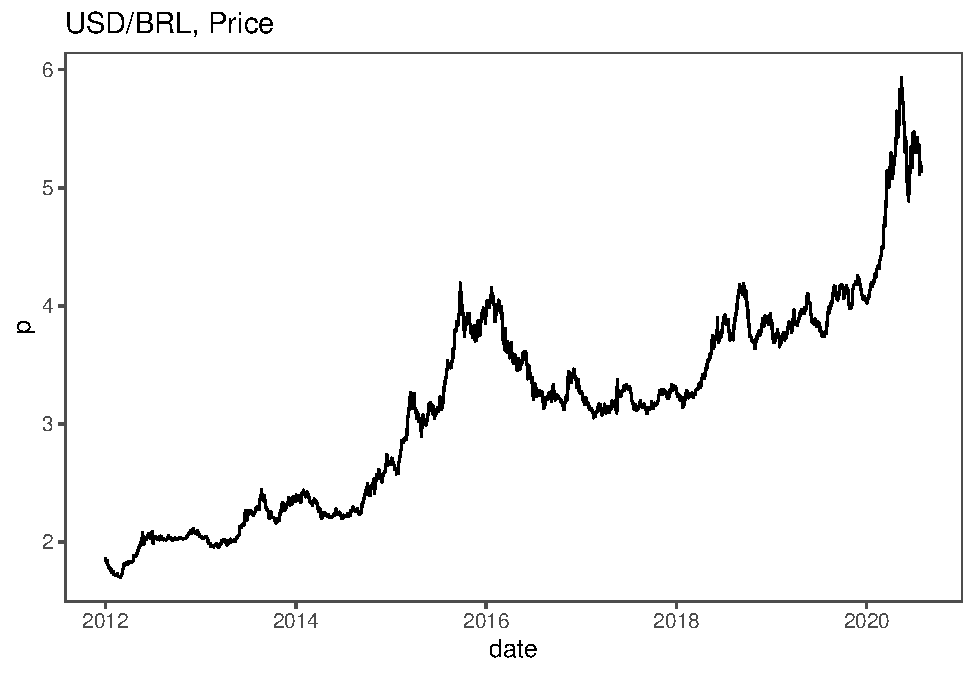
\includegraphics{Econo2_P1_files/figure-latex/plots-1} \end{center}

\begin{Shaded}
\begin{Highlighting}[]
\NormalTok{deltaplot <-}\StringTok{ }\KeywordTok{ggplot}\NormalTok{(}\DataTypeTok{data =}\NormalTok{ df, }\KeywordTok{aes}\NormalTok{(}\DataTypeTok{x =}\NormalTok{ date, }\DataTypeTok{y =}\NormalTok{ delta)) }\OperatorTok{+}\StringTok{ }\KeywordTok{geom_line}\NormalTok{() }\OperatorTok{+}\StringTok{ }
\StringTok{    }\KeywordTok{ggtitle}\NormalTok{(}\StringTok{"USD/BRL, %"}\NormalTok{) }\OperatorTok{+}\StringTok{ }\KeywordTok{theme_few}\NormalTok{()}
\NormalTok{deltaplot}
\end{Highlighting}
\end{Shaded}

\begin{center}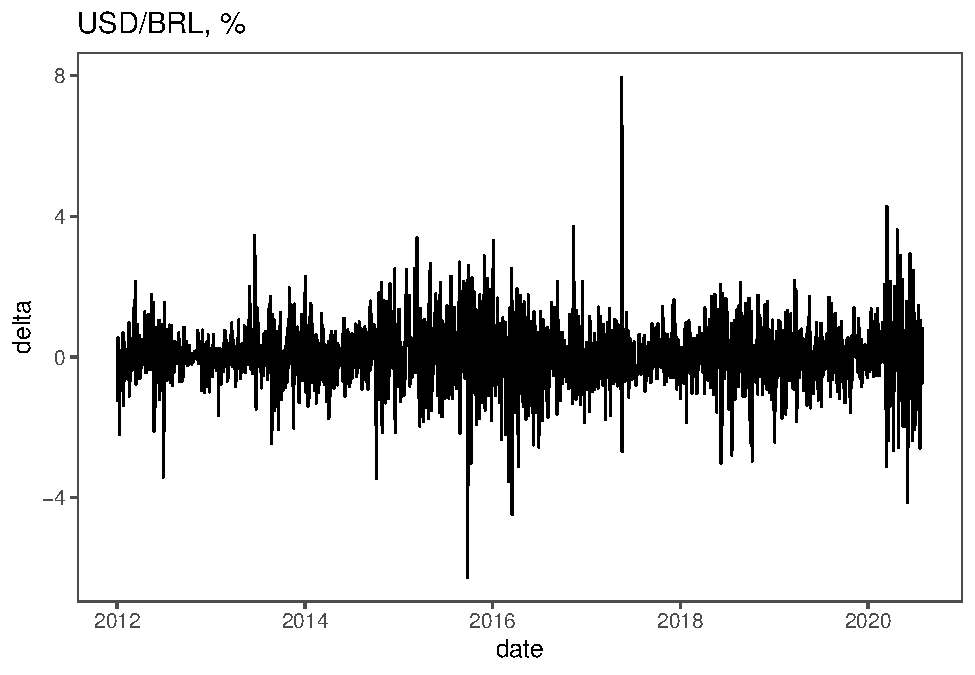
\includegraphics{Econo2_P1_files/figure-latex/plots-2} \end{center}

\begin{Shaded}
\begin{Highlighting}[]
\NormalTok{dummyplot <-}\StringTok{ }\KeywordTok{ggplot}\NormalTok{(}\DataTypeTok{data =}\NormalTok{ df, }\KeywordTok{aes}\NormalTok{(}\DataTypeTok{x =}\NormalTok{ count, }\DataTypeTok{y =}\NormalTok{ sign)) }\OperatorTok{+}\StringTok{ }\KeywordTok{geom_line}\NormalTok{() }\OperatorTok{+}\StringTok{ }
\StringTok{    }\KeywordTok{ggtitle}\NormalTok{(}\StringTok{"USD/BRL, +/-"}\NormalTok{) }\OperatorTok{+}\StringTok{ }\KeywordTok{xlim}\NormalTok{(}\DecValTok{1}\NormalTok{, }\DecValTok{200}\NormalTok{) }\OperatorTok{+}\StringTok{ }\KeywordTok{theme_few}\NormalTok{()}
\NormalTok{dummyplot}
\end{Highlighting}
\end{Shaded}

\begin{verbatim}
## Warning: Removed 1953 row(s) containing missing values (geom_path).
\end{verbatim}

\begin{center}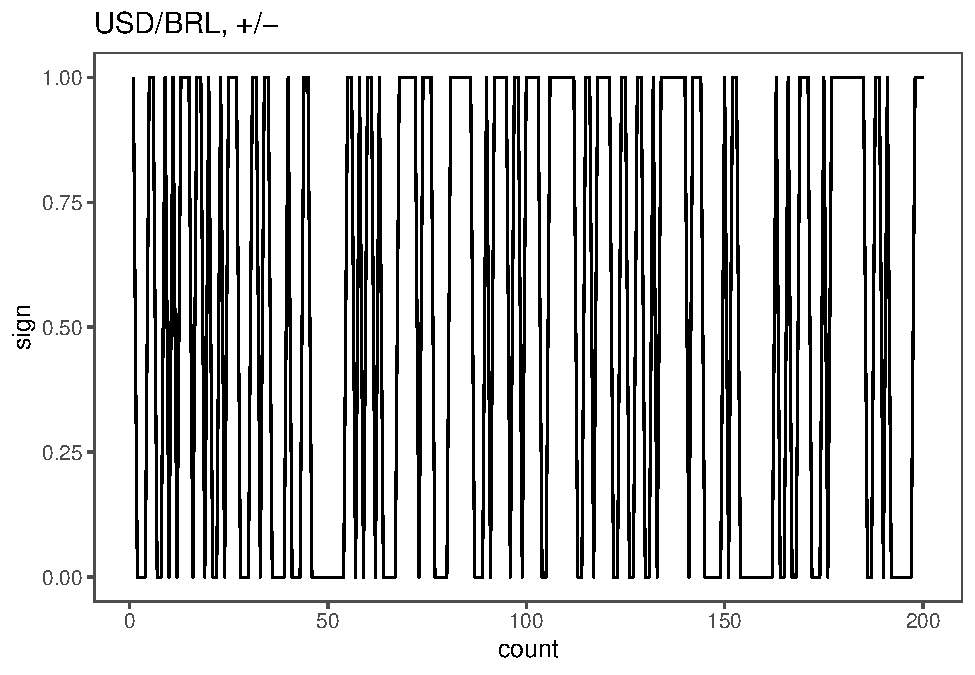
\includegraphics{Econo2_P1_files/figure-latex/plots-3} \end{center}

\begin{Shaded}
\begin{Highlighting}[]
\CommentTok{# For delta}

\NormalTok{acf_delta <-}\StringTok{ }\KeywordTok{Acf}\NormalTok{(df}\OperatorTok{$}\NormalTok{delta, }\DataTypeTok{lag.max =} \DecValTok{5000}\NormalTok{)}
\end{Highlighting}
\end{Shaded}

\begin{center}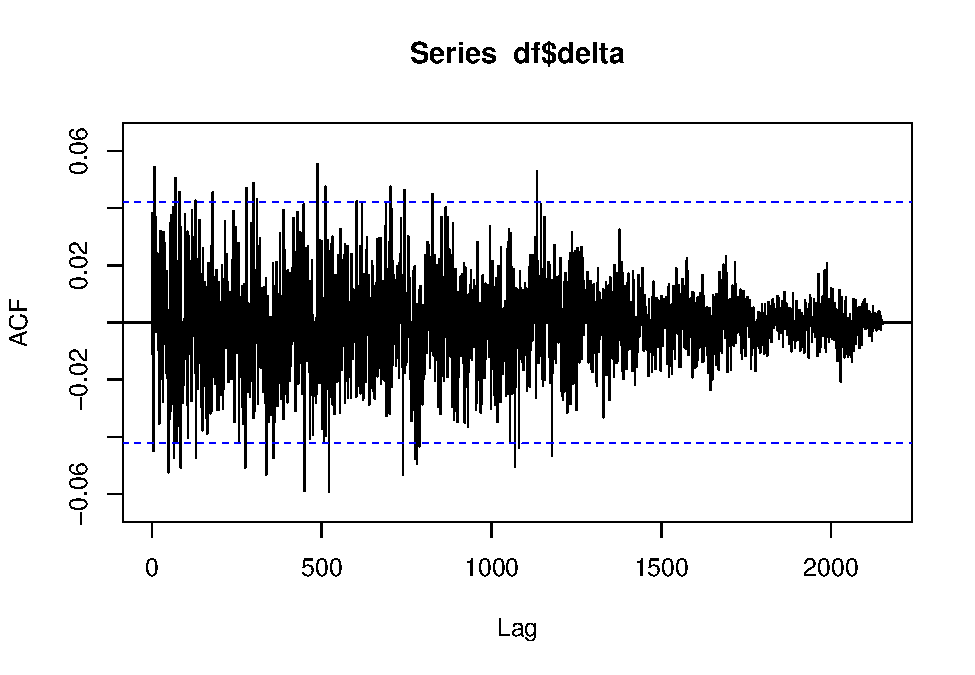
\includegraphics{Econo2_P1_files/figure-latex/plots-4} \end{center}

\begin{Shaded}
\begin{Highlighting}[]
\NormalTok{acf_test_values <-}\StringTok{ }\NormalTok{acf_delta}\OperatorTok{$}\NormalTok{acf}\OperatorTok{/}\KeywordTok{sd}\NormalTok{(acf_delta}\OperatorTok{$}\NormalTok{acf)}

\KeywordTok{head}\NormalTok{(}\KeywordTok{data.frame}\NormalTok{(acf_test_values))}
\end{Highlighting}
\end{Shaded}

\begin{verbatim}
##   acf_test_values
## 1      37.9547672
## 2       1.4506537
## 3      -0.4173129
## 4       0.2125873
## 5      -1.7053782
## 6       0.5358210
\end{verbatim}

\begin{Shaded}
\begin{Highlighting}[]
\NormalTok{facst <-}\StringTok{ }\KeywordTok{ggAcf}\NormalTok{(df}\OperatorTok{$}\NormalTok{delta, }\DataTypeTok{type =} \StringTok{"correlation"}\NormalTok{, }\DataTypeTok{lag.max =} \DecValTok{20}\NormalTok{, }
    \DataTypeTok{plot =}\NormalTok{ T) }\OperatorTok{+}\StringTok{ }\KeywordTok{theme_few}\NormalTok{()}
\NormalTok{faclt <-}\StringTok{ }\KeywordTok{ggAcf}\NormalTok{(df}\OperatorTok{$}\NormalTok{delta, }\DataTypeTok{type =} \StringTok{"correlation"}\NormalTok{, }\DataTypeTok{lag.max =} \DecValTok{5000}\NormalTok{, }
    \DataTypeTok{plot =}\NormalTok{ T) }\OperatorTok{+}\StringTok{ }\KeywordTok{theme_few}\NormalTok{()}

\NormalTok{facpst <-}\StringTok{ }\KeywordTok{ggPacf}\NormalTok{(df}\OperatorTok{$}\NormalTok{delta, }\DataTypeTok{type =} \StringTok{"correlation"}\NormalTok{, }\DataTypeTok{lag.max =} \DecValTok{100}\NormalTok{, }
    \DataTypeTok{plot =}\NormalTok{ T) }\OperatorTok{+}\StringTok{ }\KeywordTok{theme_few}\NormalTok{()}
\end{Highlighting}
\end{Shaded}

\begin{verbatim}
## Warning: Ignoring unknown parameters: type
\end{verbatim}

\begin{Shaded}
\begin{Highlighting}[]
\NormalTok{facplt <-}\StringTok{ }\KeywordTok{ggPacf}\NormalTok{(df}\OperatorTok{$}\NormalTok{delta, }\DataTypeTok{type =} \StringTok{"correlation"}\NormalTok{, }\DataTypeTok{lag.max =} \DecValTok{5000}\NormalTok{, }
    \DataTypeTok{plot =}\NormalTok{ T) }\OperatorTok{+}\StringTok{ }\KeywordTok{theme_few}\NormalTok{()}
\end{Highlighting}
\end{Shaded}

\begin{verbatim}
## Warning: Ignoring unknown parameters: type
\end{verbatim}

\begin{Shaded}
\begin{Highlighting}[]
\NormalTok{facst}
\end{Highlighting}
\end{Shaded}

\begin{center}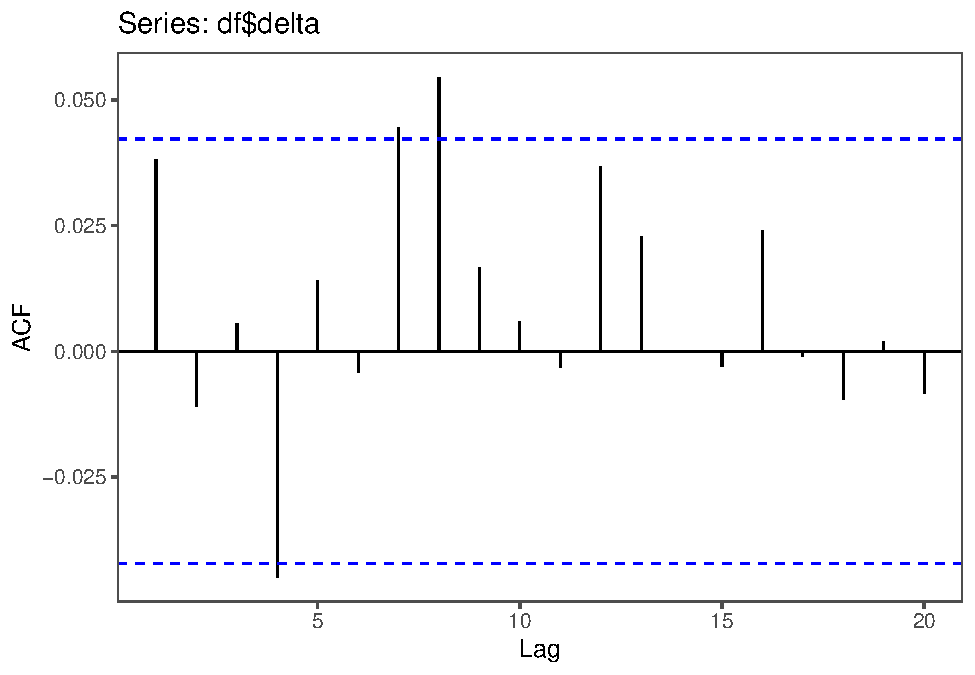
\includegraphics{Econo2_P1_files/figure-latex/plots-5} \end{center}

\begin{Shaded}
\begin{Highlighting}[]
\NormalTok{faclt}
\end{Highlighting}
\end{Shaded}

\begin{center}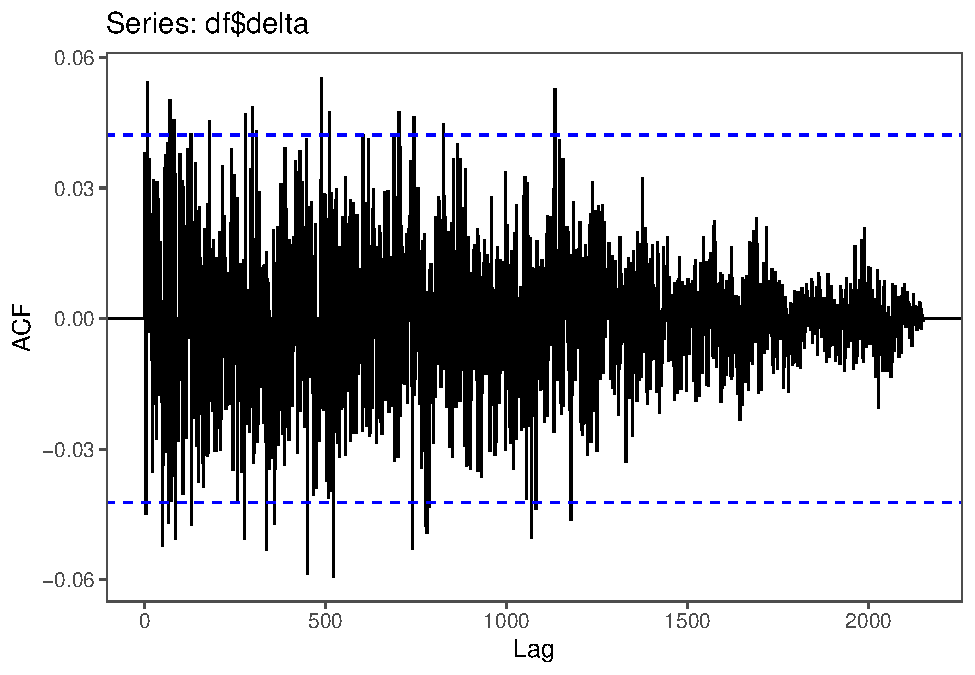
\includegraphics{Econo2_P1_files/figure-latex/plots-6} \end{center}

\begin{Shaded}
\begin{Highlighting}[]
\NormalTok{facpst}
\end{Highlighting}
\end{Shaded}

\begin{center}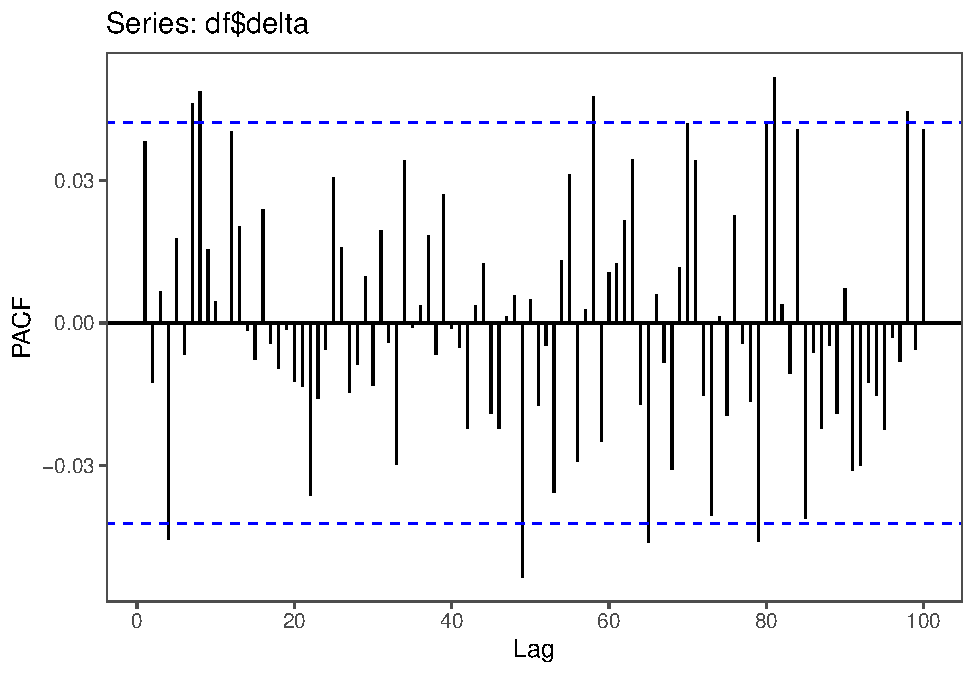
\includegraphics{Econo2_P1_files/figure-latex/plots-7} \end{center}

\begin{Shaded}
\begin{Highlighting}[]
\NormalTok{facplt}
\end{Highlighting}
\end{Shaded}

\begin{center}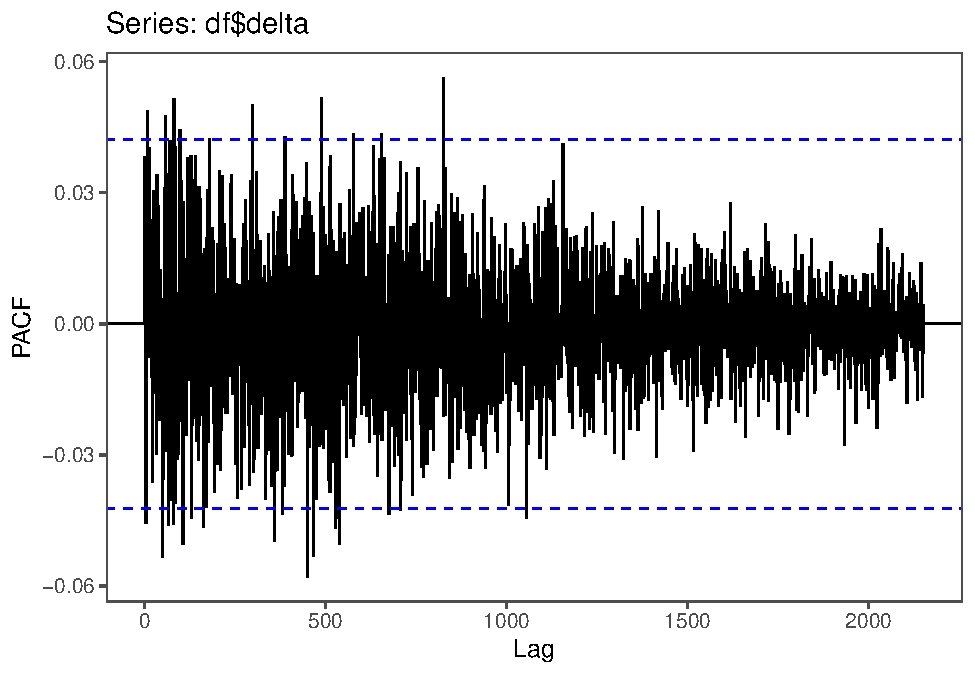
\includegraphics{Econo2_P1_files/figure-latex/plots-8} \end{center}

\begin{Shaded}
\begin{Highlighting}[]
\NormalTok{facst2 <-}\StringTok{ }\KeywordTok{ggAcf}\NormalTok{((df}\OperatorTok{$}\NormalTok{delta)}\OperatorTok{^}\DecValTok{2}\NormalTok{, }\DataTypeTok{type =} \StringTok{"correlation"}\NormalTok{, }\DataTypeTok{lag.max =} \DecValTok{20}\NormalTok{, }
    \DataTypeTok{plot =}\NormalTok{ T) }\OperatorTok{+}\StringTok{ }\KeywordTok{theme_few}\NormalTok{()}
\NormalTok{facst2}
\end{Highlighting}
\end{Shaded}

\begin{center}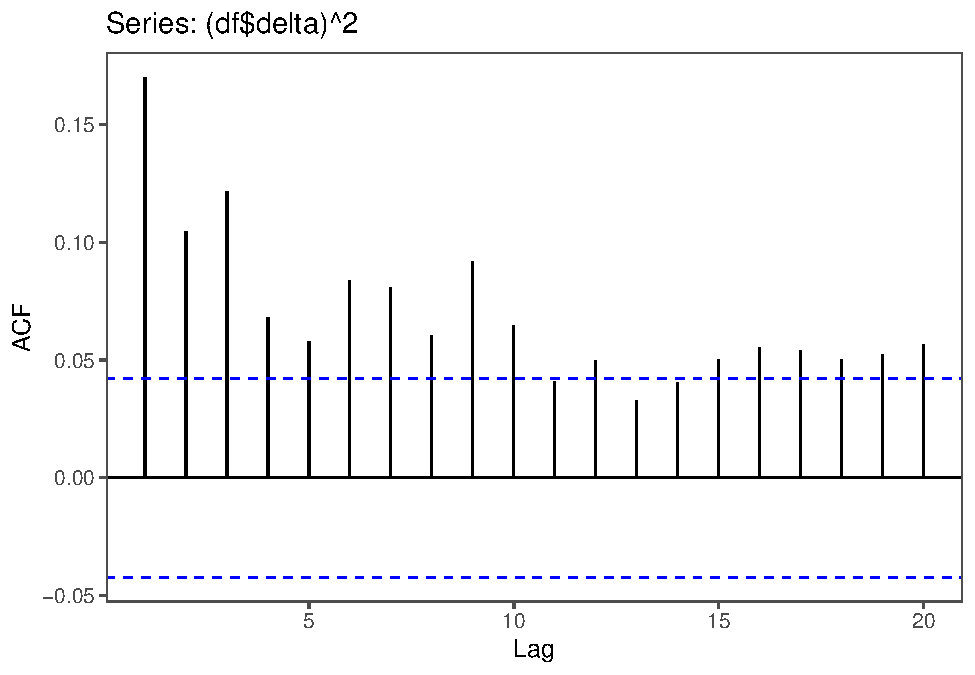
\includegraphics{Econo2_P1_files/figure-latex/plots-9} \end{center}

Let's now create our first ARMA models (equivalent to ARIMA with 2nd
argument = 0). We'll begin with the first hypothesis:
\(\mathbb{P}(+) = \mathbb{P}(-).\) Modelling this with an AR(1), we
have:

\[Sign_{t+1} = \alpha + \beta Sign_t + \varepsilon, \hspace{2em} \varepsilon \sim wn(0, \sigma^2)\]
In R, we'll use the package \emph{forecast} to construct this model:

\begin{Shaded}
\begin{Highlighting}[]
\NormalTok{AR1sign <-}\StringTok{ }\KeywordTok{Arima}\NormalTok{(df}\OperatorTok{$}\NormalTok{sign, }\DataTypeTok{order =} \KeywordTok{c}\NormalTok{(}\DecValTok{1}\NormalTok{, }\DecValTok{0}\NormalTok{, }\DecValTok{0}\NormalTok{))}
\KeywordTok{summary}\NormalTok{(AR1sign)}
\end{Highlighting}
\end{Shaded}

\begin{verbatim}
## Series: df$sign 
## ARIMA(1,0,0) with non-zero mean 
## 
## Coefficients:
##          ar1    mean
##       0.0278  0.5165
## s.e.  0.0215  0.0111
## 
## sigma^2 estimated as 0.2498:  log likelihood=-1560.63
## AIC=3127.26   AICc=3127.27   BIC=3144.28
## 
## Training set error measures:
##                        ME      RMSE       MAE  MPE MAPE     MASE          ACF1
## Training set 2.157119e-05 0.4995356 0.4990724 -Inf  Inf 1.027755 -0.0006313563
\end{verbatim}

\begin{Shaded}
\begin{Highlighting}[]
\KeywordTok{plot}\NormalTok{(AR1sign)}
\end{Highlighting}
\end{Shaded}

\begin{center}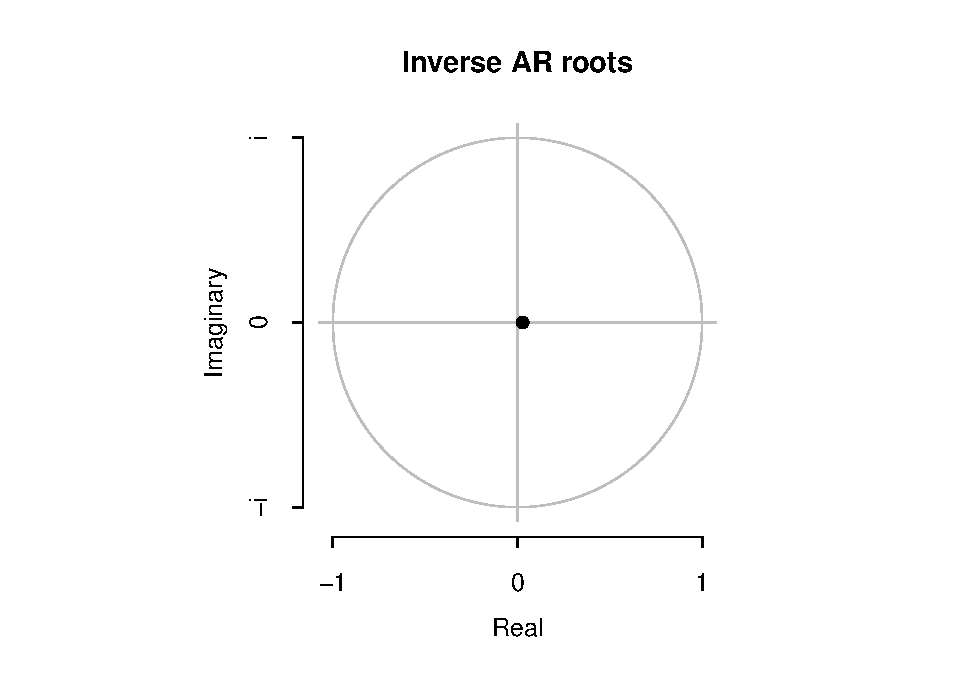
\includegraphics{Econo2_P1_files/figure-latex/AR(1)-1} \end{center}

\begin{Shaded}
\begin{Highlighting}[]
\KeywordTok{tsdisplay}\NormalTok{(AR1sign}\OperatorTok{$}\NormalTok{residuals)}
\end{Highlighting}
\end{Shaded}

\begin{center}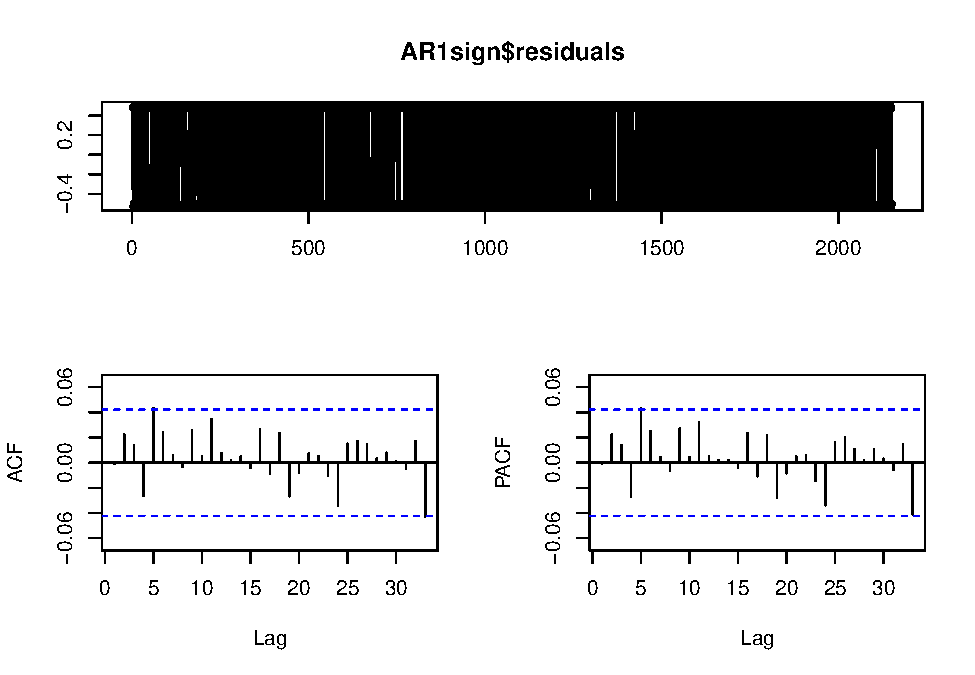
\includegraphics{Econo2_P1_files/figure-latex/AR(1)-2} \end{center}

With the results of the summary, we can now apply a hypothesis test for
our first
question.\footnote{Testing $\beta$ is equivalent to testing $\gamma$.}

\[ H_0: \beta = 0\] \[H_1: \beta \neq 0\]

\(\dfrac{\hat{ar_1} - ar_1}{s.e.(ar_1)}\):

\begin{Shaded}
\begin{Highlighting}[]
\NormalTok{AR1sign}\OperatorTok{$}\NormalTok{coef[}\DecValTok{1}\NormalTok{]}\OperatorTok{/}\KeywordTok{sqrt}\NormalTok{(AR1sign}\OperatorTok{$}\NormalTok{var.coef[}\DecValTok{1}\NormalTok{, }\DecValTok{1}\NormalTok{])}
\end{Highlighting}
\end{Shaded}

\begin{verbatim}
##      ar1 
## 1.287942
\end{verbatim}

The second hypothesis in the problem refers to the delta of the
variation: \[\mathbb{E}(\Delta | + ) \neq \mathbb{E}(\Delta | - ).\]

\[\Delta_{t+1} = \alpha + \beta Sign_t + \varepsilon, \hspace{2em} \varepsilon \sim wn(0, \sigma^2).\]

\begin{Shaded}
\begin{Highlighting}[]
\NormalTok{lmsignt <-}\StringTok{ }\KeywordTok{lm}\NormalTok{(delta }\OperatorTok{~}\StringTok{ }\KeywordTok{lag}\NormalTok{(df}\OperatorTok{$}\NormalTok{sign, }\DataTypeTok{k =} \DecValTok{1}\NormalTok{), }\DataTypeTok{data =}\NormalTok{ df)}
\KeywordTok{summary}\NormalTok{(lmsignt)}
\end{Highlighting}
\end{Shaded}

\begin{verbatim}
## 
## Call:
## lm(formula = delta ~ lag(df$sign, k = 1), data = df)
## 
## Residuals:
##     Min      1Q  Median      3Q     Max 
## -6.3285 -0.4706 -0.0060  0.4655  7.9442 
## 
## Coefficients:
##                     Estimate Std. Error t value Pr(>|t|)
## (Intercept)          0.01293    0.02811   0.460    0.646
## lag(df$sign, k = 1)  0.05802    0.03911   1.484    0.138
## 
## Residual standard error: 0.9066 on 2150 degrees of freedom
##   (1 observation deleted due to missingness)
## Multiple R-squared:  0.001023,   Adjusted R-squared:  0.000558 
## F-statistic: 2.201 on 1 and 2150 DF,  p-value: 0.1381
\end{verbatim}

\begin{Shaded}
\begin{Highlighting}[]
\KeywordTok{ggplot}\NormalTok{(df, }\KeywordTok{aes}\NormalTok{(}\DataTypeTok{x =} \KeywordTok{lag}\NormalTok{(df}\OperatorTok{$}\NormalTok{sign, }\DataTypeTok{k =} \DecValTok{1}\NormalTok{), }\DataTypeTok{y =}\NormalTok{ delta)) }\OperatorTok{+}\StringTok{ }\KeywordTok{geom_smooth}\NormalTok{(}\DataTypeTok{method =} \StringTok{"lm"}\NormalTok{)}
\end{Highlighting}
\end{Shaded}

\begin{verbatim}
## Warning: Use of `df$sign` is discouraged. Use `sign` instead.
\end{verbatim}

\begin{verbatim}
## `geom_smooth()` using formula 'y ~ x'
\end{verbatim}

\begin{verbatim}
## Warning: Removed 1 rows containing non-finite values (stat_smooth).
\end{verbatim}

\begin{center}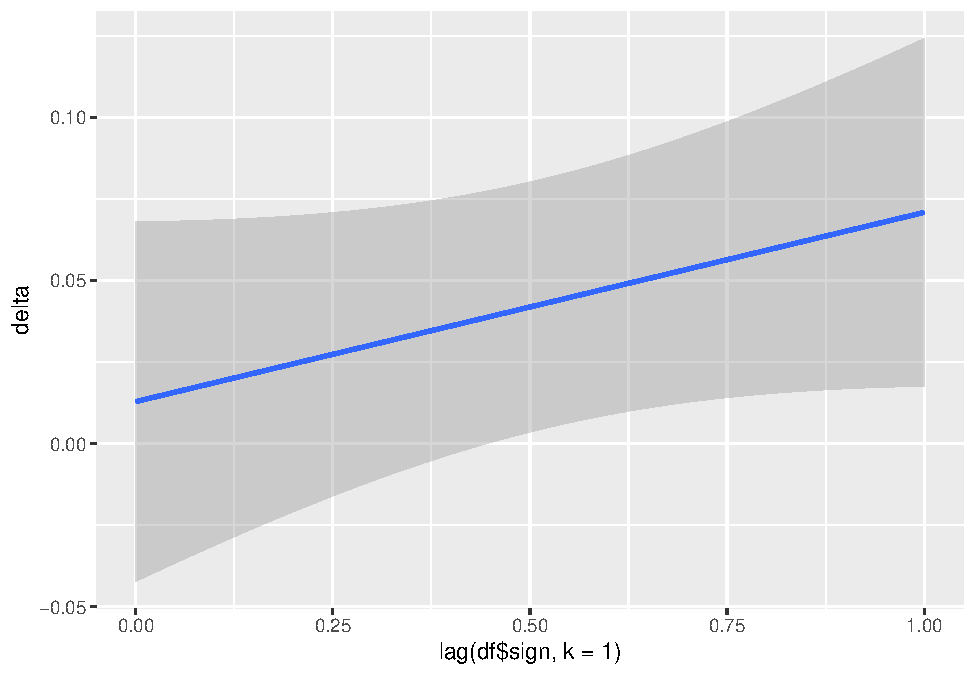
\includegraphics{Econo2_P1_files/figure-latex/lm signt-1} \end{center}

\[\Delta_{t+1} = \alpha + \beta_1 \Delta_t + \beta_2Sign_t + \varepsilon, \hspace{2em} \varepsilon \sim wn(0, \sigma^2)\]

\begin{Shaded}
\begin{Highlighting}[]
\NormalTok{AR1delta <-}\StringTok{ }\KeywordTok{Arima}\NormalTok{(df}\OperatorTok{$}\NormalTok{delta, }\DataTypeTok{order =} \KeywordTok{c}\NormalTok{(}\DecValTok{1}\NormalTok{, }\DecValTok{0}\NormalTok{, }\DecValTok{0}\NormalTok{), }\DataTypeTok{xreg =} \KeywordTok{lag}\NormalTok{(df}\OperatorTok{$}\NormalTok{sign, }
    \DataTypeTok{k =} \DecValTok{1}\NormalTok{))}
\KeywordTok{summary}\NormalTok{(AR1delta)}
\end{Highlighting}
\end{Shaded}

\begin{verbatim}
## Series: df$delta 
## Regression with ARIMA(1,0,0) errors 
## 
## Coefficients:
##          ar1  intercept    xreg
##       0.0321     0.0343  0.0166
## s.e.  0.0306     0.0351  0.0556
## 
## sigma^2 estimated as 0.8219:  log likelihood=-2840.96
## AIC=5689.93   AICc=5689.94   BIC=5712.62
## 
## Training set error measures:
##                        ME      RMSE      MAE MPE MAPE      MASE         ACF1
## Training set 1.147232e-05 0.9059341 0.643417 NaN  Inf 0.7252668 0.0003998294
\end{verbatim}

\begin{Shaded}
\begin{Highlighting}[]
\NormalTok{AR1delta}\OperatorTok{$}\NormalTok{coef[}\DecValTok{1}\NormalTok{]}\OperatorTok{/}\KeywordTok{sqrt}\NormalTok{(AR1delta}\OperatorTok{$}\NormalTok{var.coef[}\DecValTok{1}\NormalTok{, }\DecValTok{1}\NormalTok{])}
\end{Highlighting}
\end{Shaded}

\begin{verbatim}
##     ar1 
## 1.04747
\end{verbatim}

\begin{Shaded}
\begin{Highlighting}[]
\KeywordTok{plot}\NormalTok{(AR1delta)}
\end{Highlighting}
\end{Shaded}

\begin{center}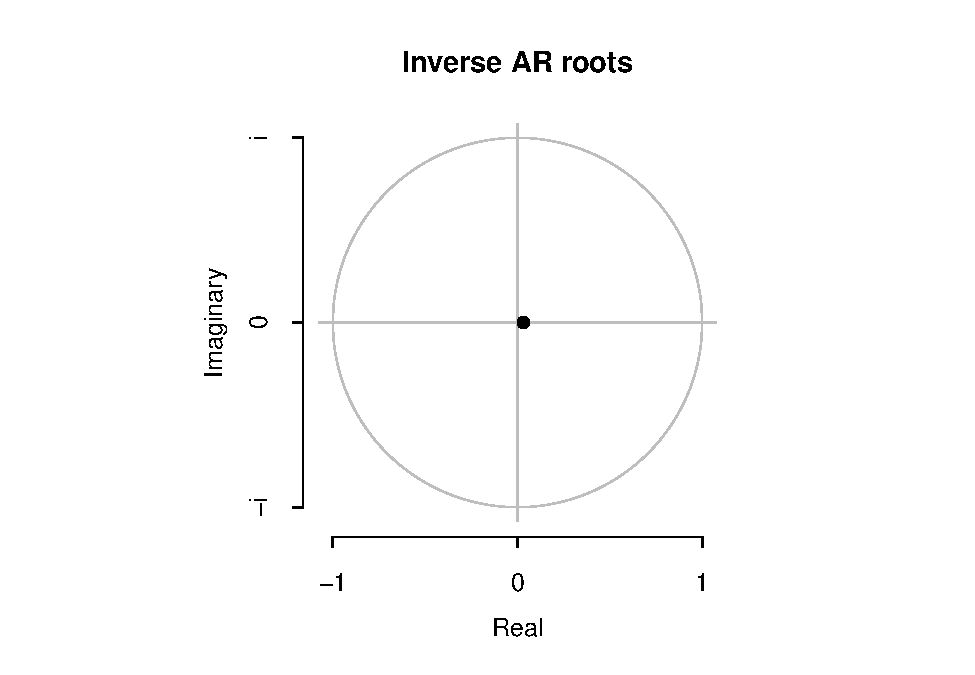
\includegraphics{Econo2_P1_files/figure-latex/delta 1-1} \end{center}

\begin{Shaded}
\begin{Highlighting}[]
\KeywordTok{tsdisplay}\NormalTok{(AR1delta}\OperatorTok{$}\NormalTok{residuals)}
\end{Highlighting}
\end{Shaded}

\begin{center}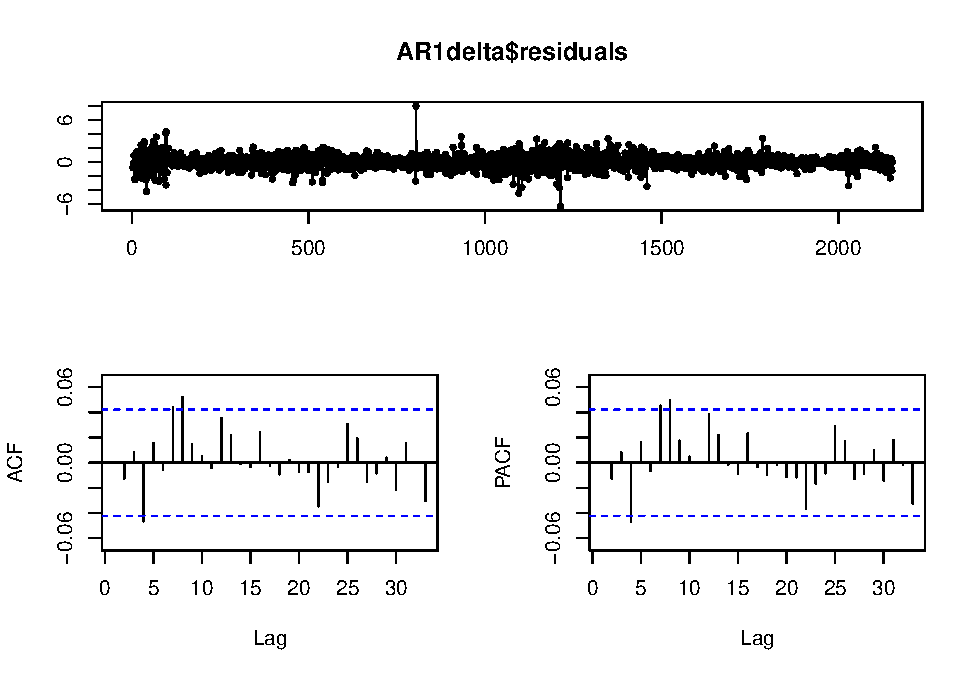
\includegraphics{Econo2_P1_files/figure-latex/delta 1-2} \end{center}

The last hypothesis in the problem refers to the variance:
\[\mathbb{E}(\Delta_{t+1}^2 | \Delta_t).\]

\[\Delta^2_{t+1} = \alpha + \beta \Delta^2_t + \varepsilon, \hspace{2em} \varepsilon \sim wn(0, \sigma^2)\]

\begin{Shaded}
\begin{Highlighting}[]
\NormalTok{AR1var <-}\StringTok{ }\KeywordTok{Arima}\NormalTok{((df}\OperatorTok{$}\NormalTok{delta)}\OperatorTok{^}\DecValTok{2}\NormalTok{, }\DataTypeTok{order =} \KeywordTok{c}\NormalTok{(}\DecValTok{1}\NormalTok{, }\DecValTok{0}\NormalTok{, }\DecValTok{0}\NormalTok{))}
\KeywordTok{summary}\NormalTok{(AR1var)}
\end{Highlighting}
\end{Shaded}

\begin{verbatim}
## Series: (df$delta)^2 
## ARIMA(1,0,0) with non-zero mean 
## 
## Coefficients:
##          ar1    mean
##       0.1701  0.8238
## s.e.  0.0212  0.0582
## 
## sigma^2 estimated as 5.026:  log likelihood=-4792.09
## AIC=9590.17   AICc=9590.18   BIC=9607.2
## 
## Training set error measures:
##                         ME     RMSE       MAE  MPE MAPE      MASE        ACF1
## Training set -6.299133e-05 2.240784 0.9197335 -Inf  Inf 0.8595655 -0.01320252
\end{verbatim}

\begin{Shaded}
\begin{Highlighting}[]
\NormalTok{AR1var}\OperatorTok{$}\NormalTok{coef[}\DecValTok{1}\NormalTok{]}\OperatorTok{/}\KeywordTok{sqrt}\NormalTok{(AR1var}\OperatorTok{$}\NormalTok{var.coef[}\DecValTok{1}\NormalTok{, }\DecValTok{1}\NormalTok{])}
\end{Highlighting}
\end{Shaded}

\begin{verbatim}
##      ar1 
## 8.011092
\end{verbatim}

\begin{Shaded}
\begin{Highlighting}[]
\KeywordTok{plot}\NormalTok{(AR1var)}
\end{Highlighting}
\end{Shaded}

\begin{center}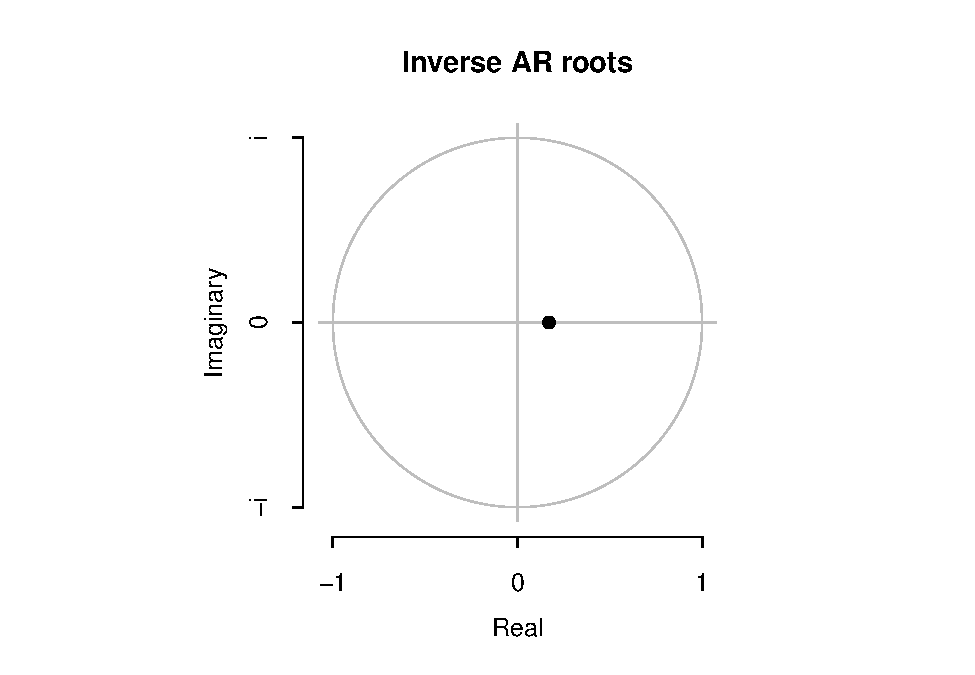
\includegraphics{Econo2_P1_files/figure-latex/var1-1} \end{center}

\begin{Shaded}
\begin{Highlighting}[]
\KeywordTok{tsdisplay}\NormalTok{(AR1var}\OperatorTok{$}\NormalTok{residuals)}
\end{Highlighting}
\end{Shaded}

\begin{center}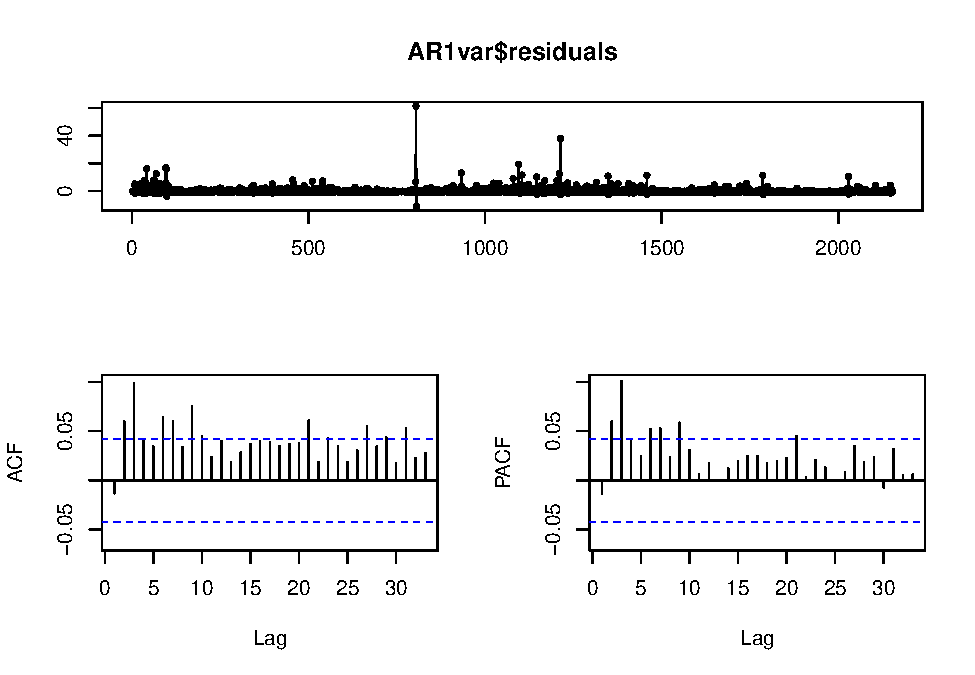
\includegraphics{Econo2_P1_files/figure-latex/var1-2} \end{center}

Now, let's run \emph{auto.arima}.

\begin{Shaded}
\begin{Highlighting}[]
\NormalTok{aadelta <-}\StringTok{ }\KeywordTok{auto.arima}\NormalTok{(df}\OperatorTok{$}\NormalTok{delta, }\DataTypeTok{stepwise =}\NormalTok{ F)}
\KeywordTok{summary}\NormalTok{(aadelta)}
\end{Highlighting}
\end{Shaded}

\begin{verbatim}
## Series: df$delta 
## ARIMA(1,0,1) with non-zero mean 
## 
## Coefficients:
##           ar1     ma1    mean
##       -0.7138  0.7506  0.0433
## s.e.   0.1486  0.1399  0.0199
## 
## sigma^2 estimated as 0.8208:  log likelihood=-2840.87
## AIC=5689.74   AICc=5689.76   BIC=5712.44
## 
## Training set error measures:
##                        ME      RMSE       MAE MPE MAPE    MASE        ACF1
## Training set 2.610156e-05 0.9053381 0.6434199 NaN  Inf 0.72527 0.003320553
\end{verbatim}

\begin{Shaded}
\begin{Highlighting}[]
\KeywordTok{plot}\NormalTok{(aadelta)}
\end{Highlighting}
\end{Shaded}

\begin{center}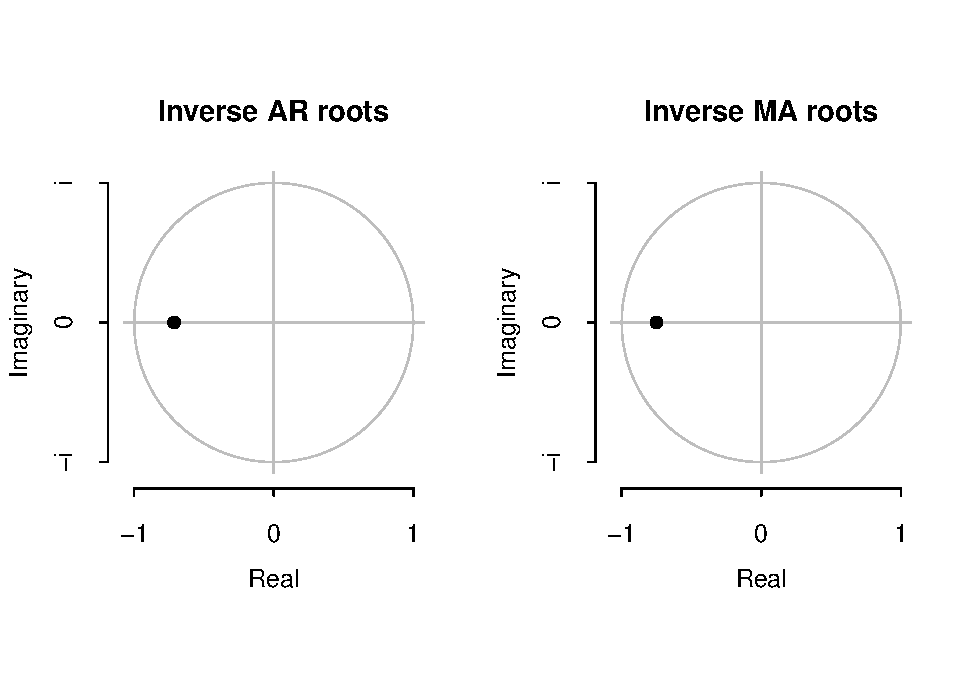
\includegraphics{Econo2_P1_files/figure-latex/auto arima-1} \end{center}

\begin{Shaded}
\begin{Highlighting}[]
\KeywordTok{tsdisplay}\NormalTok{(aadelta}\OperatorTok{$}\NormalTok{residuals)}
\end{Highlighting}
\end{Shaded}

\begin{center}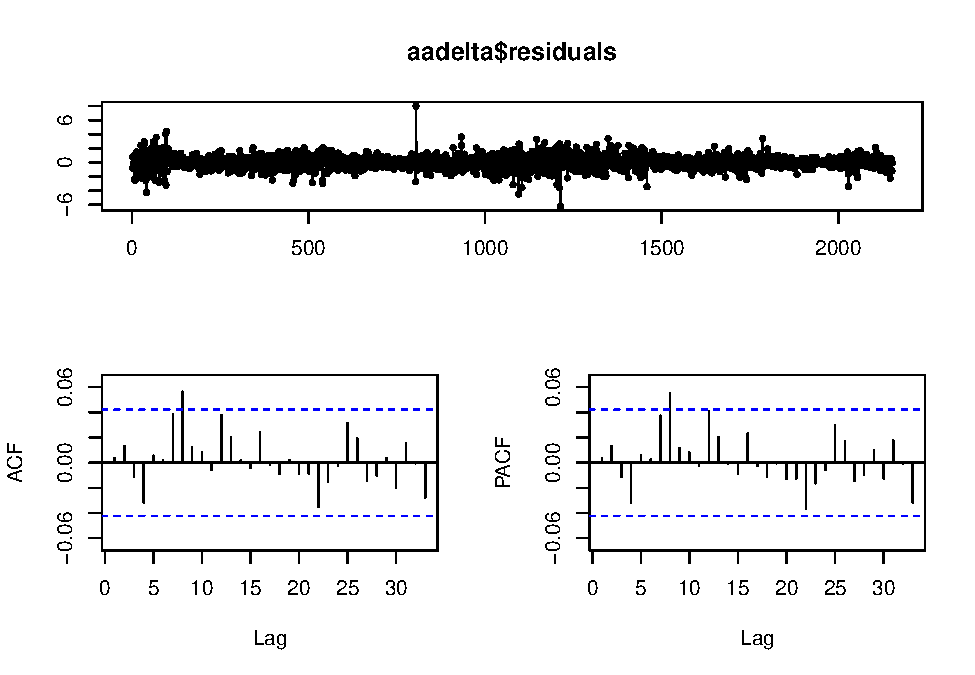
\includegraphics{Econo2_P1_files/figure-latex/auto arima-2} \end{center}

\begin{Shaded}
\begin{Highlighting}[]
\NormalTok{aasign <-}\StringTok{ }\KeywordTok{auto.arima}\NormalTok{(df}\OperatorTok{$}\NormalTok{sign, }\DataTypeTok{stepwise =}\NormalTok{ F)}
\KeywordTok{summary}\NormalTok{(aasign)}
\end{Highlighting}
\end{Shaded}

\begin{verbatim}
## Series: df$sign 
## ARIMA(0,0,0) with non-zero mean 
## 
## Coefficients:
##         mean
##       0.5165
## s.e.  0.0108
## 
## sigma^2 estimated as 0.2498:  log likelihood=-1561.46
## AIC=3126.91   AICc=3126.92   BIC=3138.26
## 
## Training set error measures:
##                         ME      RMSE       MAE  MPE MAPE     MASE       ACF1
## Training set -2.382602e-13 0.4997281 0.4994563 -Inf  Inf 1.028545 0.02773919
\end{verbatim}

\begin{Shaded}
\begin{Highlighting}[]
\KeywordTok{plot}\NormalTok{(aasign)}
\end{Highlighting}
\end{Shaded}

\begin{verbatim}
## Warning in plot.Arima(aasign): No roots to plot
\end{verbatim}

\begin{center}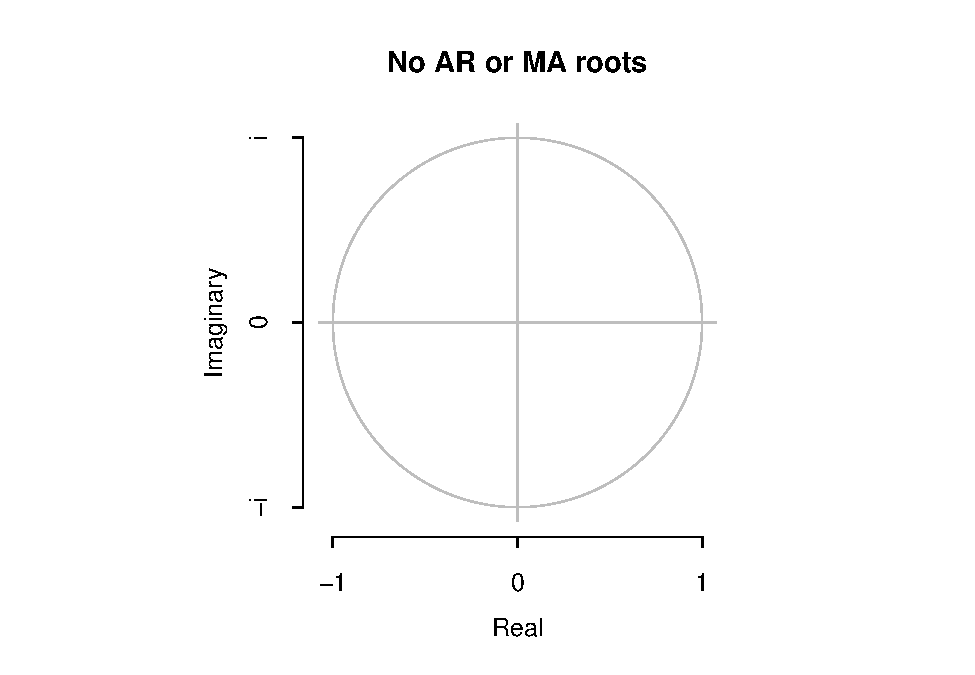
\includegraphics{Econo2_P1_files/figure-latex/auto arima-3} \end{center}

\begin{Shaded}
\begin{Highlighting}[]
\KeywordTok{tsdisplay}\NormalTok{(aasign}\OperatorTok{$}\NormalTok{residuals)}
\end{Highlighting}
\end{Shaded}

\begin{center}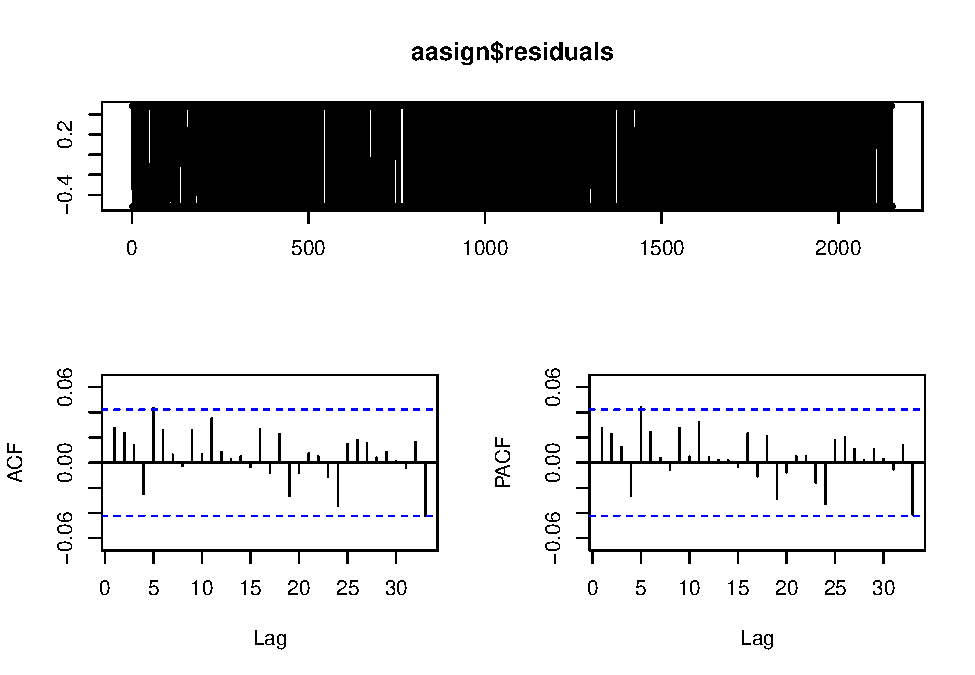
\includegraphics{Econo2_P1_files/figure-latex/auto arima-4} \end{center}

\begin{Shaded}
\begin{Highlighting}[]
\NormalTok{aavar <-}\StringTok{ }\KeywordTok{auto.arima}\NormalTok{((df}\OperatorTok{$}\NormalTok{delta)}\OperatorTok{^}\DecValTok{2}\NormalTok{, }\DataTypeTok{stepwise =}\NormalTok{ F)}
\KeywordTok{summary}\NormalTok{(aavar)}
\end{Highlighting}
\end{Shaded}

\begin{verbatim}
## Series: (df$delta)^2 
## ARIMA(0,1,4) 
## 
## Coefficients:
##           ma1      ma2     ma3      ma4
##       -0.8662  -0.0671  0.0228  -0.0641
## s.e.   0.0215   0.0284  0.0280   0.0214
## 
## sigma^2 estimated as 4.892:  log likelihood=-4761.22
## AIC=9532.45   AICc=9532.48   BIC=9560.82
## 
## Training set error measures:
##                       ME     RMSE       MAE  MPE MAPE      MASE         ACF1
## Training set -0.02170361 2.209213 0.8904046 -Inf  Inf 0.8321553 0.0001189823
\end{verbatim}

\begin{Shaded}
\begin{Highlighting}[]
\KeywordTok{plot}\NormalTok{(aavar)}
\end{Highlighting}
\end{Shaded}

\begin{center}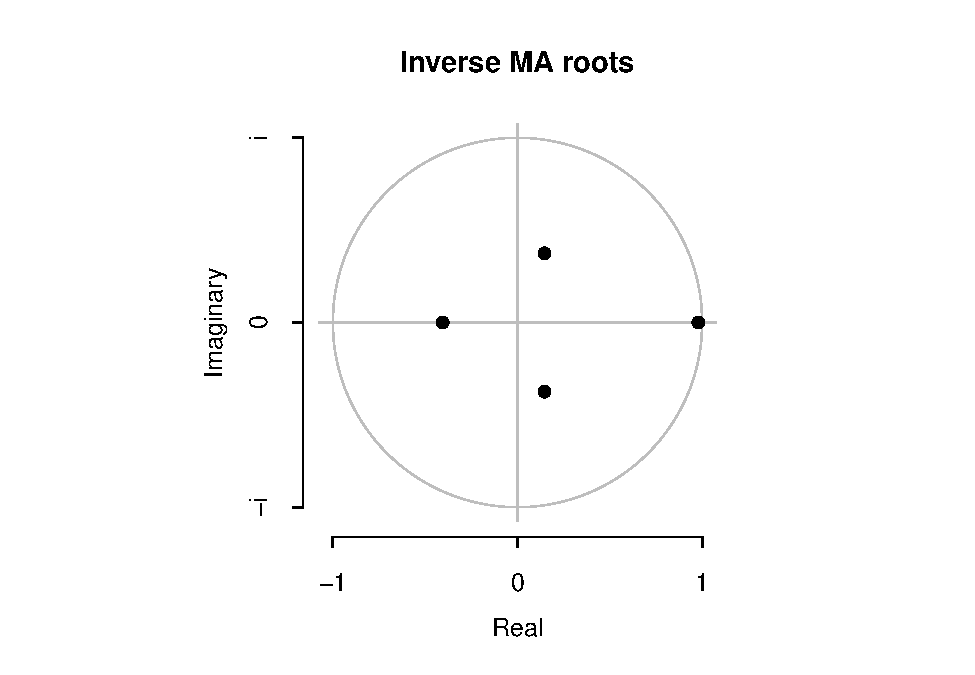
\includegraphics{Econo2_P1_files/figure-latex/auto arima-5} \end{center}

\begin{Shaded}
\begin{Highlighting}[]
\KeywordTok{tsdisplay}\NormalTok{(aasign}\OperatorTok{$}\NormalTok{residuals)}
\end{Highlighting}
\end{Shaded}

\begin{center}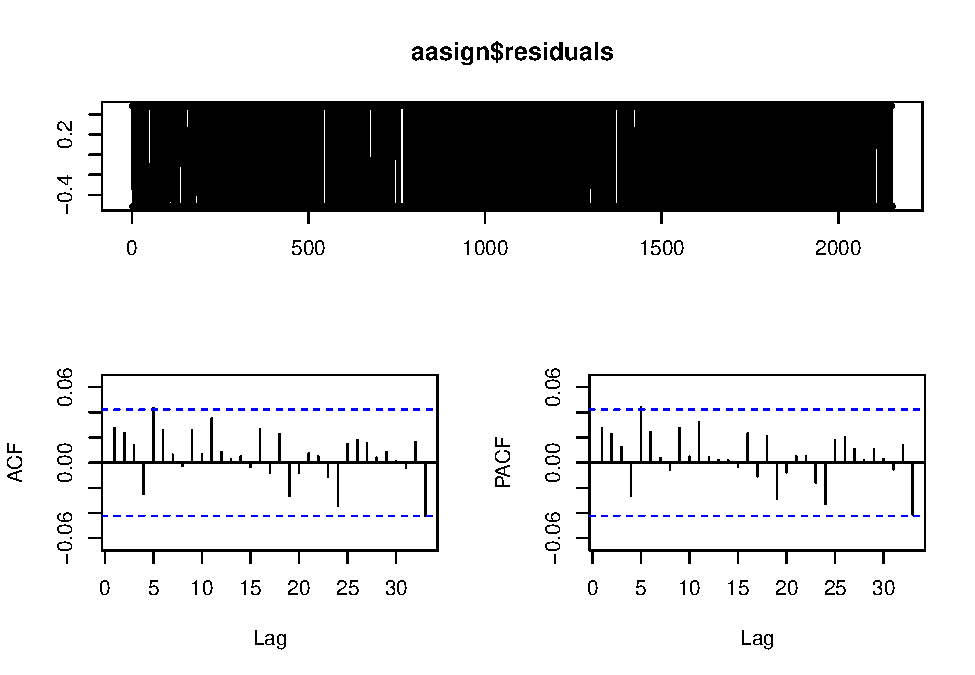
\includegraphics{Econo2_P1_files/figure-latex/auto arima-6} \end{center}

\begin{Shaded}
\begin{Highlighting}[]
\NormalTok{aardelta <-}\StringTok{ }\KeywordTok{auto.arima}\NormalTok{(df}\OperatorTok{$}\NormalTok{delta, }\DataTypeTok{max.q =} \DecValTok{0}\NormalTok{, }\DataTypeTok{stepwise =}\NormalTok{ F)}
\KeywordTok{summary}\NormalTok{(aardelta)}
\end{Highlighting}
\end{Shaded}

\begin{verbatim}
## Series: df$delta 
## ARIMA(1,0,0) with non-zero mean 
## 
## Coefficients:
##          ar1    mean
##       0.0382  0.0433
## s.e.  0.0215  0.0203
## 
## sigma^2 estimated as 0.8215:  log likelihood=-2842.26
## AIC=5690.52   AICc=5690.53   BIC=5707.54
## 
## Training set error measures:
##                         ME      RMSE       MAE MPE MAPE      MASE         ACF1
## Training set -1.464203e-05 0.9059233 0.6434299 NaN  Inf 0.7252813 0.0004805619
\end{verbatim}

\begin{Shaded}
\begin{Highlighting}[]
\KeywordTok{plot}\NormalTok{(aardelta)}
\end{Highlighting}
\end{Shaded}

\begin{center}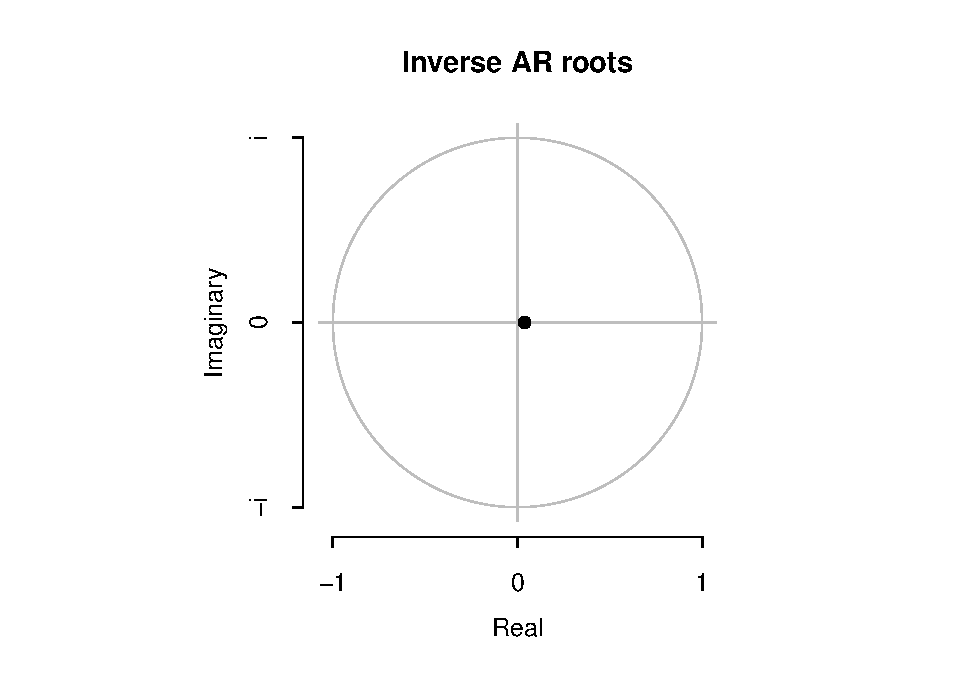
\includegraphics{Econo2_P1_files/figure-latex/auto arima-7} \end{center}

\begin{Shaded}
\begin{Highlighting}[]
\KeywordTok{tsdisplay}\NormalTok{(aardelta}\OperatorTok{$}\NormalTok{residuals)}
\end{Highlighting}
\end{Shaded}

\begin{center}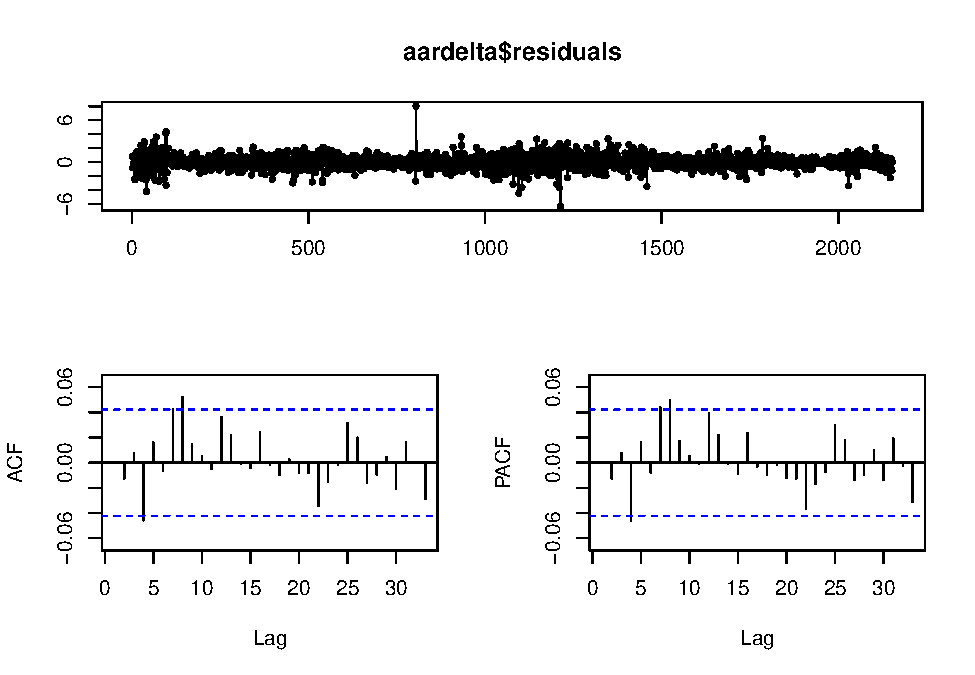
\includegraphics{Econo2_P1_files/figure-latex/auto arima-8} \end{center}

\begin{Shaded}
\begin{Highlighting}[]
\NormalTok{aarsign <-}\StringTok{ }\KeywordTok{auto.arima}\NormalTok{(df}\OperatorTok{$}\NormalTok{sign, }\DataTypeTok{max.q =} \DecValTok{0}\NormalTok{, }\DataTypeTok{stepwise =}\NormalTok{ F)}
\KeywordTok{summary}\NormalTok{(aarsign)}
\end{Highlighting}
\end{Shaded}

\begin{verbatim}
## Series: df$sign 
## ARIMA(0,0,0) with non-zero mean 
## 
## Coefficients:
##         mean
##       0.5165
## s.e.  0.0108
## 
## sigma^2 estimated as 0.2498:  log likelihood=-1561.46
## AIC=3126.91   AICc=3126.92   BIC=3138.26
## 
## Training set error measures:
##                         ME      RMSE       MAE  MPE MAPE     MASE       ACF1
## Training set -2.382602e-13 0.4997281 0.4994563 -Inf  Inf 1.028545 0.02773919
\end{verbatim}

\begin{Shaded}
\begin{Highlighting}[]
\KeywordTok{plot}\NormalTok{(aarsign)}
\end{Highlighting}
\end{Shaded}

\begin{verbatim}
## Warning in plot.Arima(aarsign): No roots to plot
\end{verbatim}

\begin{center}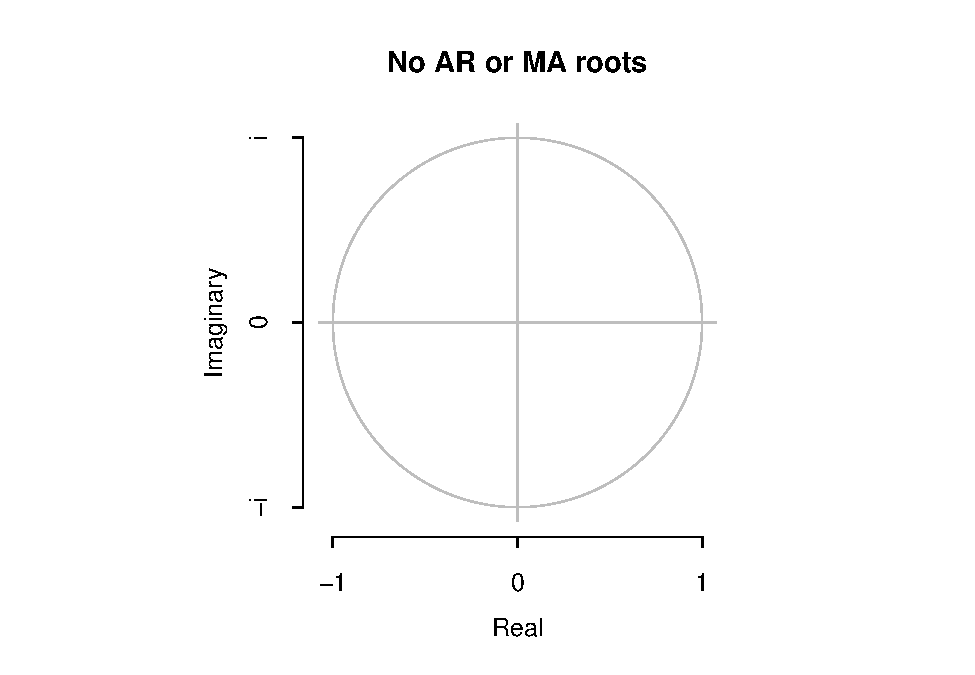
\includegraphics{Econo2_P1_files/figure-latex/auto arima-9} \end{center}

\begin{Shaded}
\begin{Highlighting}[]
\KeywordTok{tsdisplay}\NormalTok{(aarsign}\OperatorTok{$}\NormalTok{residuals)}
\end{Highlighting}
\end{Shaded}

\begin{center}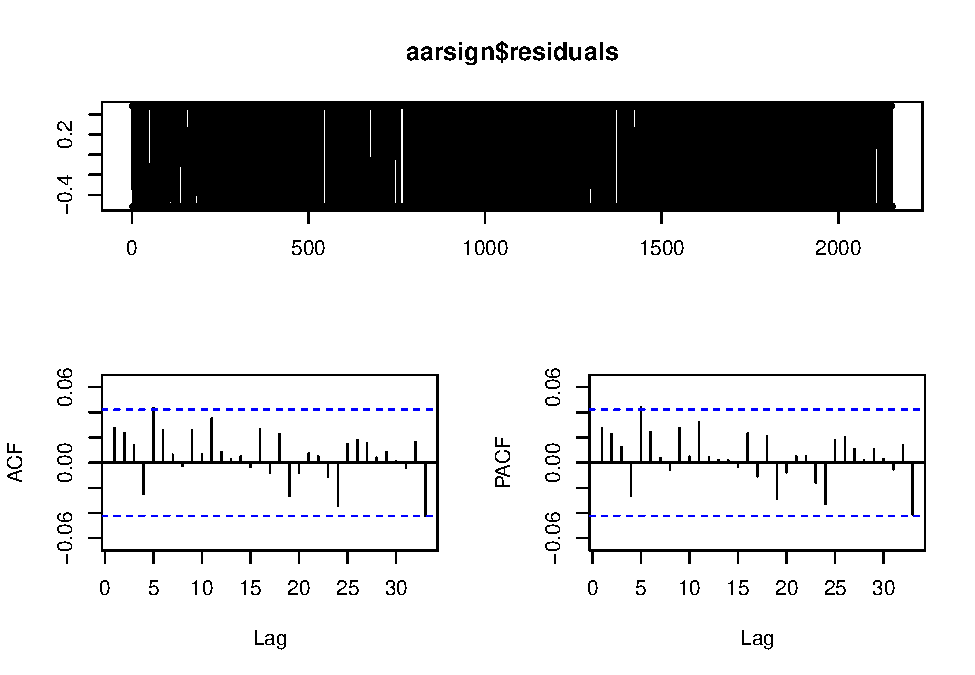
\includegraphics{Econo2_P1_files/figure-latex/auto arima-10} \end{center}

\begin{Shaded}
\begin{Highlighting}[]
\NormalTok{aarvar <-}\StringTok{ }\KeywordTok{auto.arima}\NormalTok{((df}\OperatorTok{$}\NormalTok{delta)}\OperatorTok{^}\DecValTok{2}\NormalTok{, }\DataTypeTok{max.q =} \DecValTok{0}\NormalTok{, }\DataTypeTok{stepwise =}\NormalTok{ F)}
\KeywordTok{summary}\NormalTok{(aarvar)}
\end{Highlighting}
\end{Shaded}

\begin{verbatim}
## Series: (df$delta)^2 
## ARIMA(5,1,0) 
## 
## Coefficients:
##           ar1      ar2      ar3      ar4      ar5
##       -0.7420  -0.5845  -0.4042  -0.2873  -0.1687
## s.e.   0.0213   0.0259   0.0274   0.0258   0.0212
## 
## sigma^2 estimated as 5.465:  log likelihood=-4878.95
## AIC=9769.89   AICc=9769.93   BIC=9803.94
## 
## Training set error measures:
##                         ME     RMSE       MAE  MPE MAPE      MASE       ACF1
## Training set -3.234587e-05 2.334504 0.9170278 -Inf  Inf 0.8570369 -0.0239684
\end{verbatim}

\begin{Shaded}
\begin{Highlighting}[]
\KeywordTok{plot}\NormalTok{(aarvar)}
\end{Highlighting}
\end{Shaded}

\begin{center}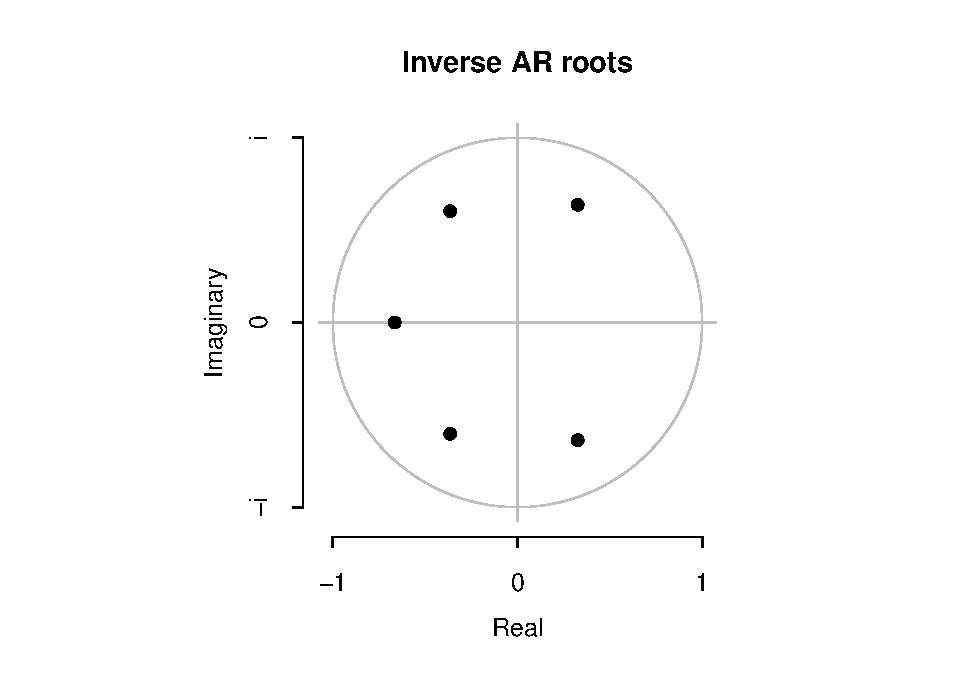
\includegraphics{Econo2_P1_files/figure-latex/auto arima-11} \end{center}

\begin{Shaded}
\begin{Highlighting}[]
\KeywordTok{tsdisplay}\NormalTok{(aarvar}\OperatorTok{$}\NormalTok{residuals)}
\end{Highlighting}
\end{Shaded}

\begin{center}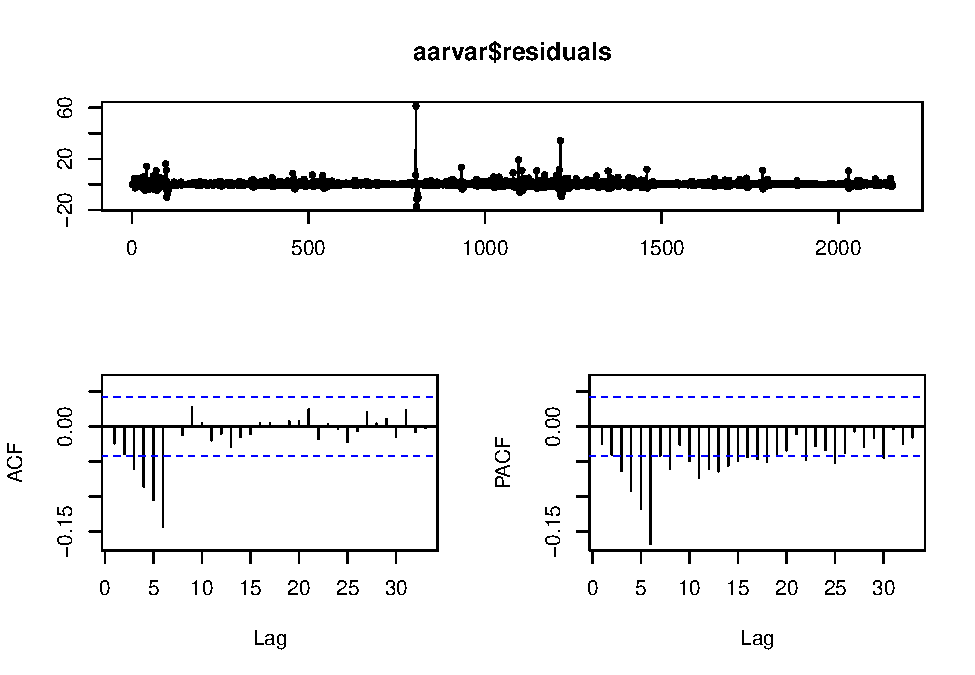
\includegraphics{Econo2_P1_files/figure-latex/auto arima-12} \end{center}

\[ \Delta_{t+1} = c + \beta \Delta_t + \varepsilon\]

\begin{Shaded}
\begin{Highlighting}[]
\NormalTok{AR1_}\DecValTok{2}\NormalTok{ <-}\StringTok{ }\KeywordTok{Arima}\NormalTok{(df}\OperatorTok{$}\NormalTok{delta, }\DataTypeTok{order =} \KeywordTok{c}\NormalTok{(}\DecValTok{1}\NormalTok{, }\DecValTok{0}\NormalTok{, }\DecValTok{0}\NormalTok{))}

\KeywordTok{summary}\NormalTok{(AR1_}\DecValTok{2}\NormalTok{)}
\end{Highlighting}
\end{Shaded}

\begin{verbatim}
## Series: df$delta 
## ARIMA(1,0,0) with non-zero mean 
## 
## Coefficients:
##          ar1    mean
##       0.0382  0.0433
## s.e.  0.0215  0.0203
## 
## sigma^2 estimated as 0.8215:  log likelihood=-2842.26
## AIC=5690.52   AICc=5690.53   BIC=5707.54
## 
## Training set error measures:
##                         ME      RMSE       MAE MPE MAPE      MASE         ACF1
## Training set -1.464203e-05 0.9059233 0.6434299 NaN  Inf 0.7252813 0.0004805619
\end{verbatim}

\begin{Shaded}
\begin{Highlighting}[]
\KeywordTok{confint}\NormalTok{(AR1_}\DecValTok{2}\NormalTok{, }\DataTypeTok{level =} \FloatTok{0.95}\NormalTok{)}
\end{Highlighting}
\end{Shaded}

\begin{verbatim}
##                  2.5 %     97.5 %
## ar1       -0.003988796 0.08042284
## intercept  0.003511958 0.08308440
\end{verbatim}

\end{document}